% Physical Review E — self-contained APS RevTeX 4.2 bundle
\ifdefined\pdfobjcompresslevel \pdfobjcompresslevel=0 \fi
\documentclass[%
 twocolumn,
 superscriptaddress,
 amsmath,amssymb,
 aps,
 pre,
 floatfix,
]{revtex4-2}

\usepackage{graphicx}
\usepackage{dcolumn}
\usepackage{bm}
\usepackage{amsthm}
\usepackage[breaklinks=true,hidelinks]{hyperref}
\hypersetup{
  pdftitle={Closer is not sharper: bounded information and an observability horizon at a noisy saddle-node},
  pdfauthor={Alexander Sokol},
}

\graphicspath{{figures/}}

\newtheorem{theorem}{Theorem}
\newtheorem{lemma}{Lemma}
\newtheorem{proposition}{Proposition}
\newtheorem{corollary}{Corollary}

\newcommand{\dd}{\mathrm{d}}
\newcommand{\Ifish}{\mathcal{I}}
\newcommand{\Leff}{\mathcal{L}}
%% dimensionless ramp rate 2 eps / D.  A single symbol: a three-letter roman
%% word inside displayed equations reads badly in APS style.
\newcommand{\Sig}{\hat\varepsilon}
\newcommand{\E}{\mathbb{E}}

\begin{document}

\title{Closer is not sharper: bounded information and an
  observability horizon at a noisy saddle-node}

\author{Alexander Sokol}
\email[Contact author: ]{alex.sokol.research@gmail.com}
\affiliation{Independent Researcher, Limassol, Cyprus}

\date{\today}

\begin{abstract}
Early-warning indicators for critical transitions are analyzed almost universally with an Ornstein--Uhlenbeck (OU) surrogate, which near a saddle-node predicts that the information a \emph{single} observation carries about the control parameter $r$ --- the distance to threshold, at noise strength $D$ --- diverges as $|r|^{-2}$.  It does not.  Conditioned on non-explosion --- the stopping time the dynamics themselves supply --- it stays bounded, and is not even maximized at threshold: the snapshot Fisher information $\Ifish$ peaks one noise scale out, at $|r|\simeq0.88\,(D/2)^{2/3}$, and declines by $10\%$ to a universal value $0.4875(1)$ in units of $(D/2)^{-4/3}$, rounding the divergence off at the scale $|r|\sim D^{2/3}$.  That bound is a per-snapshot statement and not a limit on learning: the full record carries $E[\tau]/D$ with $\tau$ the escape time, unbounded in observation time.  Comparing the two exactly locates the surrogate's error.  For a continuous record the OU \emph{mean} channel reproduces the path bound $1/D$ per unit time identically, and the entire spurious divergence sits in the \emph{variance} channel --- the statistic early-warning practice actually computes, so what it inherits is an artifact of the linearization and not a property of the process.  What closes instead is the set of parameter values an ensemble survives to report on: the accumulated escape hazard integrates exactly, giving a closed-form observability horizon that \emph{recedes} from threshold as the ramp slows and that, for dimensionless ramp rates $\Sig=2\varepsilon/D\lesssim0.10$, a typical trajectory never carries into the regime where the surrogate fails.  Through a projection of the applied noise covariance onto the center direction, the horizon predicts the distance from the fold at which a two-box thermohaline model collapses to $2.8\%$ at the slower of two ramp rates and $7.4\%$ at the faster, with no fitted parameters.
\end{abstract}

\keywords{Critical phenomena, Stochastic processes, Bifurcation, Nonlinear dynamics}

\maketitle

%==============================================================================
\section{\label{sec:intro}Introduction}
%==============================================================================

Critical slowing down motivates the standard early-warning signals (EWS) for critical transitions --- rising variance and lag-1 autocorrelation as a control parameter approaches a bifurcation~\cite{Scheffer2009,Dakos2012,Kuehn2011}.  The empirical record of these indicators is mixed~\cite{Dakos2024,Ditlevsen2023}, the finite-data limits to detection are severe~\cite{Boettiger2012,Grziwotz2023}, and this has motivated spectral and machine-learning detectors~\cite{Bury2020,Bury2021} as well as indicators built from the full windowed distribution rather than from its low-order moments~\cite{Prokopenko2011}, for which the natural language is information geometry~\cite{Amari2000,Nielsen2020}.  That language has recently been developed for bifurcations in its own right~\cite{DaSilva2026}, but as a Riemannian geometry of parameter space; the object here is the Cram\'er--Rao bound on estimating one parameter, which is a different use of the same Fisher matrix.

Nearly all of this rests on a single surrogate.  One linearizes about the slowly moving stable fixed point and treats the windowed law as the resulting Ornstein--Uhlenbeck (OU) Gaussian.  For a saddle-node approached as $r\to0^-$ this gives a stationary variance $v_{\mathrm{OU}}=D/(4\sqrt{|r|})$ that grows without bound, and a per-observation Fisher information about $r$ that diverges as $|r|^{-2}$.  Read literally, the surrogate promises unlimited resolution: the closer the system comes to threshold, the more sharply a fixed observation window should locate it.

\paragraph{The two questions.}
That promise invites two questions which must be answered together, because either alone is misleading.  \emph{Is the divergence real?}  And \emph{is the regime in which it appears reachable?}  A system driven toward a saddle-node in noise generally escapes before the bifurcation is attained~\cite{Ashwin2012,Ritchie2016,BerglundGentz2006}, so a statement about the limit $|r|\to0$ may be a statement about states of vanishing probability.  A divergence that is real but unreachable has no observational content; a reachable regime in which the divergence fails would invalidate the surrogate where it is actually used.  Only by settling both does one learn what limits early warning.

Answering either question requires committing to a conditioned law --- the law of the system \emph{given that it has not yet tipped} --- and that commitment must be argued rather than assumed.  We emphasize this because the tempting alternative is not equivalent to the correct one, and the difference is not small (Sec.~\ref{sec:law}).

\paragraph{What is new.}
Stated before anything else, so that a reader can locate the claim without reconstructing it: the new content is (i) the Fisher information of the law conditioned on explosion --- that it is bounded, that it is \emph{not} maximized at threshold but one noise scale away, and the universal constants $\Ifish_s(0)=0.4875(1)$ and $\max\Ifish_s=0.5425$ that go with it; (ii) the argument that the conditioning must be explosion rather than the unstable fixed point, killing there changing the rate by a factor $2.012$ and manufacturing a spurious support edge; and (iii) the observability statement --- that the region in which the surrogate is quantitatively wrong lies inside the region a typical ramped trajectory has already vacated, for ramp rates below Eq.~(\ref{eq:sigcont}), together with the exact channel decomposition~(\ref{eq:channels}) that locates the surrogate's error in its variance term alone.  Everything else below is either rederived from the references named above so that Sec.~\ref{sec:sat} can use it, or --- in the cases of the census rule of Sec.~\ref{sec:sat}\,D and the noise projection of Sec.~\ref{sec:stommel} --- a validated application of a result that belongs to the survival-analysis and stochastic-reduction literatures respectively, as those sections state at the point of use.

\paragraph{What is old here, conceded in full.}
The escape side of this problem has a long history, and none of it is ours.  For a metastable state approached along a control parameter $\eta$ measured from its critical value, the activation barrier scales as $\eta^{3/2}$; this is the standard reading of ramped switching experiments in Josephson junctions and nanomagnets, traced to Kurkij\"arvi~\cite{Kurkijarvi1972} and Fulton and Dunkelberger~\cite{FultonDunkelberger1974} on the experimental side and to Dykman and Krivoglaz~\cite{DykmanKrivoglaz1980}, Victora~\cite{Victora1989} and Tretiakov \emph{et al.}~\cite{Tretiakov2003} on the theoretical, with the escape-field distribution under a steady ramp computed by Garg~\cite{Garg1995}.  Dykman and co-workers made the exponent explicit as a critical exponent, $|\ln W|\propto\eta^{\xi}$ with $\xi=3/2$ in the adiabatic regime, and identified the crossover to $\xi=2$ when the drive is fast enough that the state cannot follow~\cite{DykmanGoldingRyvkine2004,RyvkineDykmanGolding2004}.  Escape statistics for a noisy normal form swept through a saddle-node were formulated and solved numerically by Miller and Shaw~\cite{MillerShaw2012}.  Herbert and Bouchet~\cite{HerbertBouchet2017} obtained the result this paper uses: for the ramped stochastic fold the quasi-static Kramers hazard integrates in closed form, giving a Gumbel first-passage law whose typical escape location scales as $[\ln(1/\varepsilon)]^{2/3}$.  Hathcock and Sethna~\cite{HathcockSethna2021} completed the picture at the other end, giving a renormalization-group scaling description valid at \emph{arbitrary} barrier height, including the barrierless limit where Kramers' formula fails.

Everything in Sec.~\ref{sec:horizon} --- the $\tfrac43|s|^{3/2}$ barrier, the Kramers rate, the exactly integrable hazard, the Gumbel law and the $[\ln(1/\varepsilon)]^{2/3}$ escape location --- belongs to that literature.  We rederive it because Sec.~\ref{sec:sat} needs it in a particular form and because the conditioned setting used here supplies the constants directly in scaled variables, and we fix the correspondence with Ref.~\cite{HerbertBouchet2017} exactly (Table~\ref{tab:dictionary}) so that no step of the comparison rests on inspection.  The reader should take those results as established.  What is new begins where the escape law is used as an input rather than produced as an output.

\paragraph{Where this ends up.}
The concrete test is in Sec.~\ref{sec:stommel}, and a reader who wants the physical payoff before the stochastic calculus can read it early: for a two-box thermohaline model with a genuine saddle-node, the horizon derived here predicts the point at which the model actually collapses to $2.8\%$ at the slower of two ramp rates and $7.4\%$ at the faster, with no fitted parameters, the noise entering only through a projection of the applied covariance onto the center direction.  Sections~\ref{sec:law}--\ref{sec:lag} are what that prediction is made of.

\paragraph{Approach.}
Our method throughout is to obtain results in closed form and to use numerics only to verify them, never to define them.  This is not stylistic.  A numerically tabulated threshold cannot be extrapolated, cannot be checked against an independent calculation without reproducing the entire pipeline, and hides the parametric structure that makes a result portable to other systems.  Where a quantity genuinely does not close --- and three of them do not --- we say so explicitly and identify the operator whose spectrum they are.

\paragraph{Results.}
Five, of which the first three are the paper's substance and the last two are applications of it.
\begin{enumerate}

\item \textbf{The snapshot information stays bounded, and is not maximized at threshold.}  The Fisher information of the conditioned law does not diverge; it peaks at $0.5425$ one noise scale out, at $s=-0.88$, then \emph{declines} by $10\%$ to $\Ifish_s(0)=0.4875(1)$.  The OU $|r|^{-2}$ is rounded off at $|r|\sim D^{2/3}$, and the closest approach is not the most informative one (Sec.~\ref{sec:sat}\,A).  Two prerequisites are part of the result rather than lemmas to it: the conditioning must be explosion, since killing at the unstable fixed point changes the escape rate by a factor $2.012$ and manufactures a spurious parameter-dependent support edge; and the conditioned law has a flux tail $\rho\to\lambda/(s+y^2)$, so its moments diverge and every moment-based indicator carries an implicit observation cutoff that the Fisher information does not (Sec.~\ref{sec:law}).

\item \textbf{That bound is not a limit on learning, and the surrogate's error has a specific address.}  The information in the full record is $E[\tau]/D$ --- one line of Girsanov~\cite{LiptserShiryaev2001b}, holding for any additive-noise diffusion with an unknown drift offset and carrying no saddle-node content --- so proximity to the fold is informationally neutral per unit surviving time.  What the comparison buys is Eq.~(\ref{eq:channels}): for a continuous record the OU \emph{mean} channel reproduces that bound identically, and the entire spurious divergence sits in the \emph{variance} channel, which is the statistic early-warning practice computes (Sec.~\ref{sec:sat}\,B).

\item \textbf{For $\Sig\lesssim0.10$, a typical trajectory never observes the surrogate fail.}  Here $\Sig=2\varepsilon/D$ is the ramp rate made dimensionless by the noise, the only combination the problem depends on (Lemma~\ref{thm:scaling}).  Below that rate the median horizon of the \emph{simulated} ramped process --- not of the quasi-static closed form, which overstates the threshold by $20\%$ --- lies outside the regime in which OU is quantitatively wrong, and the containment survives varying both conventions on which it rests.  Two restrictions are stated rather than buried.  The bound is on typical members, not all of them: at the fastest rate considered, a fifth of the ensemble does reach the failure region.  And $\Sig\simeq0.10$ is stricter than both the domain~(\ref{eq:domain}) of the closed form and the adiabaticity limit of Sec.~\ref{sec:kz}, so there is a band of ramp rates, a factor $2.3$ wide, in which the closed form is defined but containment fails --- and a factor $2.01$ of it over which the quasi-static reading also still holds (Sec.~\ref{sec:sat}\,C; Table~\ref{tab:thresholds}).

\item \textbf{A parameter-free prediction of a physical model's collapse point.}  For a two-box thermohaline model with a genuine saddle-node, the horizon predicts the measured collapse to $2.8\%$ at the slower of two ramp rates and $7.4\%$ at the faster, with nothing fitted.  A three-way error decomposition attributes the difference to the adiabatic lag at the faster rate and the Kramers prefactor at the slower, the dimensional reduction costing about $1\%$ at both (Sec.~\ref{sec:stommel}).  Carrying the horizon out of one dimension requires the noise projection $D_{\mathrm{eff}}=b^2f^{\mathsf T}\Sigma\Sigma^{\mathsf T}f$, which is standard stochastic center-manifold theory and which we claim only as the step at which a reader applying Eq.~(\ref{eq:horizon_r}) to their own model will otherwise use the wrong eigenvector.

\item \textbf{Two exact by-products, neither of them about folds.}  An adiabatic correction $\mu_1=\langle\phi,\partial_s\rho\rangle$ to the quasi-static hazard, validated by a Hellmann--Feynman identity and showing that the non-adiabatic regime is never entered (Sec.~\ref{sec:lag}); and an observational design rule --- one binary census of a ramped ensemble carries $64.8\%$ of the information in the full tipping-time record, optimally taken when $79.68\%$ has tipped.  The design rule is a proportional-hazards fact that holds for \emph{any} increasing cumulative hazard, not a consequence of the fold's exact integrability, and is classical in the survival-analysis literature; we include it because it is useful here and appears not to be known in the tipping literature (Sec.~\ref{sec:sat}\,D).

\end{enumerate}

%==============================================================================
\section{\label{sec:model}Model and scaling reduction}
%==============================================================================

The ramped noisy fold is
\begin{equation}
\label{eq:fold}
\dd x=(r+x^2)\,\dd t+\sqrt D\,\dd W_t,\qquad \dot r=\varepsilon>0,\quad r<0,
\end{equation}
with stable fixed point $x^\ast=-\sqrt{|r|}$ and unstable fixed point $x^{\ast\ast}=+\sqrt{|r|}$.  Equation~(\ref{eq:fold}) is the normal form for a saddle-node with additive noise; Sec.~\ref{sec:stommel} and Appendix~\ref{app:cmf} address what happens when a physical system is reduced to it.

Linearizing about $x^\ast$ gives $\mu_{\mathrm{OU}}=-\sqrt{|r|}$ and $v_{\mathrm{OU}}=D/(4\sqrt{|r|})$, hence a per-observation Fisher information
\begin{equation}
\label{eq:iou}
\Ifish^{\mathrm{OU}}
=\frac{(\dd\mu/\dd r)^2}{v}+\frac{(\dd v/\dd r)^2}{2v^2}
=\frac{1}{D\sqrt{|r|}}+\frac{1}{8r^2},
\end{equation}
whose second term is the advertised $|r|^{-2}$ divergence.

Because $r+x^2\sim x^2$ at large $x$, the deterministic flow reaches $+\infty$ in finite time; the same is true of Eq.~(\ref{eq:fold}) almost surely.  The process \emph{explodes}.  This is not a pathology to be regularized away --- it is the mathematical content of ``the system has run away'', and Sec.~\ref{sec:law} shows that it is what fixes the conditioned law.

\begin{lemma}[Scaling reduction]
\label{thm:scaling}
With $\ell=(D/2)^{1/3}$ and $x=\ell y$,
\begin{equation}
\label{eq:generator}
\tfrac D2\partial_x^2+(r+x^2)\partial_x
=\ell\bigl[\partial_y^2+(s+y^2)\partial_y\bigr],
\qquad s\equiv \frac{r}{(D/2)^{2/3}},
\end{equation}
so the generator depends on $(r,D)$ only through $s$, up to the overall rate $\ell$.  Consequently $\lambda=\ell\,\tilde\lambda(s)$, lengths scale as $\ell$, and every Fisher information about $r$ scales as
\begin{equation}
\label{eq:Iscale}
\Ifish_r=(D/2)^{-4/3}\,\Ifish_s(s),
\end{equation}
with $\tilde\lambda$ and $\Ifish_s$ universal functions of $s$ alone.
\end{lemma}

\noindent\textit{Proof.} Appendix~\ref{app:scaling}. $\square$

Lemma~\ref{thm:scaling} is a change of variables, standard for the fold and not new here: Ref.~\cite{HerbertBouchet2017} performs the equivalent reduction in the opposite direction, normalizing the ramp rather than the diffusion, and Eq.~(\ref{eq:dictionary}) below is the exact transformation between the two.  We state it because it fixes every $D$-dependence in what follows without further computation, and because it converts the three constants that remain numerical (Sec.~\ref{sec:num}) into universal numbers rather than fitted parameters.  Table~\ref{tab:collapse} verifies the collapse to eight significant figures across a $64\times$ range in $D$.  Because Lemma~\ref{thm:scaling} is a change of variables, that collapse is exact by construction; the table tests the implementation, not the physics, and we present it as such.

\begin{table}[b]
\caption{\label{tab:collapse}%
Scaling collapse: the scaled escape rate depends only on $s$, not on $D$ and $r$ separately.  Computed by the eigenproblem of Sec.~\ref{sec:num}.}
\begin{ruledtabular}
\begin{tabular}{lrr}
$D$ & $s$ & $\lambda/(D/2)^{1/3}$ \\
\colrule
$0.09$    & $-0.5$ & $0.18335138$ \\
$0.72$    & $-0.5$ & $0.18335138$ \\
$0.01125$ & $-0.5$ & $0.18335138$ \\
$0.09$    & $-2.0$ & $0.00953406$ \\
$0.72$    & $-2.0$ & $0.00953406$ \\
$0.01125$ & $-2.0$ & $0.00953406$ \\
\end{tabular}
\end{ruledtabular}
\end{table}

%==============================================================================
\section{\label{sec:law}Which conditioned law?}
%==============================================================================

A system observed before it tips is described by a law conditioned on not having tipped.  The definition of ``tipped'' therefore fixes the law, and different definitions give genuinely different answers.  This section argues for one definition and quantifies the cost of the alternative.

\subsection{The explosion time is the natural stopping time}

Equation~(\ref{eq:fold}) supplies a stopping time without ambiguity.  Trajectories explode in finite time; the explosion time is measurable with respect to the dynamics alone, requires no externally chosen threshold, and the events ``the system has run away'' and ``the trajectory has exploded'' coincide.  We therefore take the conditioned law to be the quasi-stationary law with respect to explosion --- the Yaglom limit~\cite{MeleardVillemonais2012,Collet2013} --- namely the principal eigenfunction of the forward generator,
\begin{equation}
\label{eq:killed}
\tfrac D2\rho''-\partial_y\bigl[(s+y^2)\rho\bigr]=-\lambda\,\rho ,
\end{equation}
normalizable, with all killing carried by the outgoing probability flux at $y\to+\infty$.

\emph{A convention, stated here rather than later.}  Equations~(\ref{eq:killed}) and~(\ref{eq:tail}) are written in the scaled variables $(y,s)$ of Lemma~\ref{thm:scaling}, in which the diffusion coefficient has been normalized to the coefficient of $y^2$; that is, $D/2=1$.  We retain the symbol $D/2$ in these two equations only to keep the current $J$ recognizable, and every numerical quantity reported for the scaled operator uses $D/2=1$.  The same convention governs the conjugation $\rho=e^{(sy+y^3/3)/D}g$ in Appendix~\ref{app:num}.

\subsection{The cost of killing at the unstable fixed point}

The tempting alternative is to kill at $x^{\ast\ast}$, which is a point of no return \emph{deterministically}.  With noise it is not: a trajectory just beyond $x^{\ast\ast}$ returns with positive probability, and in the scaling region the barrier has all but vanished, so such excursions are common rather than exceptional.  The two choices are not equivalent, in two distinct ways.

\emph{The rate.}  Solving Eq.~(\ref{eq:killed}) with an absorbing cutoff at $y_R$ and increasing $y_R$, the escape rate converges rapidly: at $s=-0.5$, $\lambda=0.1833513840$ agrees to eight significant digits for $y_R\ge4$ ($0.183351385$ at $y_R=4$ against $0.183351389$ at $y_R=16$).  The cutoff is thus a numerical device with a controlled limit, not a modeling choice.  Killing at $x^{\ast\ast}$, by contrast, gives
\begin{equation}
\label{eq:xssratio}
\frac{\lambda(x^{\ast\ast})}{\lambda(\infty)}=2.012\ (s=-0.5),\qquad 1.793\ (s=-2),
\end{equation}
a factor of two --- not an exponentially small correction [Fig.~\ref{fig:cond}(a)].

\emph{The support.}  Killing at $x^{\ast\ast}$ also endows the law with a support edge that moves with the parameter, at unbounded speed $|\dd x^{\ast\ast}/\dd r|=1/(2\sqrt{|r|})$ as $r\to0^-$.  A density vanishing at a parameter-dependent boundary is the textbook non-regular estimation problem~\cite{IbragimovHasminskii,AkahiraTakeuchi}, for which the Fisher information diverges logarithmically for reasons that have nothing to do with the physics of the approach to threshold.  An analysis built on that conditioning would report a spurious divergence and attribute it to critical slowing down.  None of this survives the correct conditioning: under Eq.~(\ref{eq:killed}) the support is all of $\mathbb{R}$, independent of $s$, and the family is regular.

\subsection{The flux tail and the divergence of moments}

Far beyond the well the drift dominates and the law settles into flux balance.  Equating the probability current $J=-\tfrac D2\rho'+(s+y^2)\rho$ to the total killing rate gives the following.

\begin{proposition}[Flux tail]
\label{prop:tail}
The principal solution of Eq.~(\ref{eq:killed}) satisfies
\begin{equation}
\label{eq:tail}
\rho(y)\longrightarrow \frac{\lambda}{s+y^2}\qquad(y\to\infty).
\end{equation}
\end{proposition}

\noindent\textit{Proof.} Appendix~\ref{app:tail}. $\square$

Equation~(\ref{eq:tail}) is confirmed to $2\%$ by $y=10$ [Fig.~\ref{fig:cond}(b)] and independently by direct simulation (Sec.~\ref{sec:num}).  Neither Proposition~\ref{prop:tail} nor its consequence below is new at $s=0$.  Ornigotti \emph{et al.}~\cite{Ornigotti2018} study the quasi-stationary law of the unstable cubic potential --- Eq.~(\ref{eq:killed}) at $s=0$ --- observe that the natural boundary conditions leave a non-vanishing probability current at the escaping end, and make the divergence of the moments the starting point of their paper, proposing the quasi-stationary description in their place.  What is added here is the $s$-dependence, which is what the ramp requires; the comparison with killing at $x^{\ast\ast}$; and the Fisher information of the resulting family.

\begin{corollary}[Moments diverge]
\label{cor:moments}
$\rho$ is integrable, hence a probability density; but $\int y\rho\,\dd y$ and $\int y^2\rho\,\dd y$ diverge.  The conditioned law has no finite mean and no finite variance.
\end{corollary}

This is not a technicality.  Variance and lag-1 autocorrelation --- the two workhorse indicators --- are moment functionals.  Corollary~\ref{cor:moments} says that for this model their population values do not exist: any number reported for them is a property of the observation cutoff (the largest excursion the instrument records, or the window length), not of the process.  Two studies using different cutoffs will measure different ``variances'' of the same system and both will be right.

We therefore use the Fisher information, which requires no cutoff, and which by the data-processing inequality~\cite{CoverThomas2006} upper-bounds the information carried by \emph{every} statistic computable from the same observation, moment-based or otherwise.  A limit stated in Fisher information is thus a limit on all indicators at once, not on a particular choice --- provided one is careful about what ``the same observation'' means, a point Sec.~\ref{sec:sat}\,B makes precise.

\begin{figure*}[t]
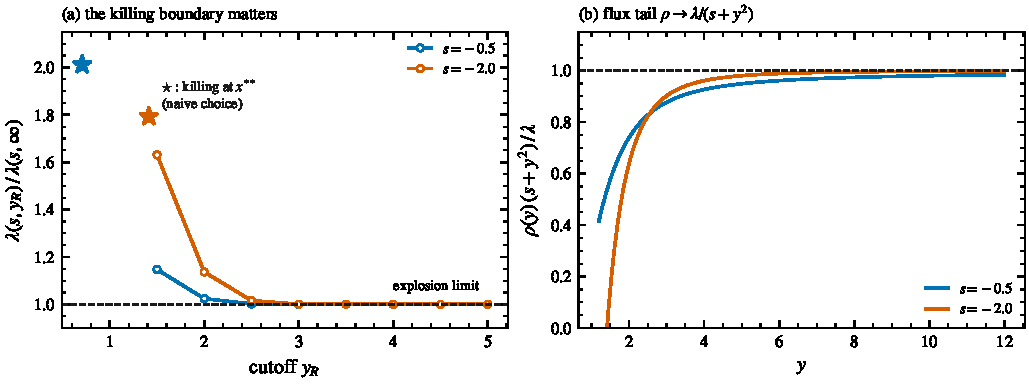
\includegraphics[width=\textwidth]{fig_conditioned.pdf}
\caption{\label{fig:cond}%
(a)~The escape rate converges as the numerical cutoff $y_R$ moves out, defining the explosion limit; stars mark killing at $x^{\ast\ast}$, which overestimates $\lambda$ by a factor $2.012$ at $s=-0.5$.
(b)~The flux tail of Eq.~(\ref{eq:tail}).}
\end{figure*}

%==============================================================================
\section{\label{sec:horizon}The escape law and the observability horizon}
%==============================================================================

This section assembles the horizon.  Its ingredients are prior art, as set out in the introduction; the assembly, and the reading of the result as a statement about which parameter values an ensemble survives to report on, is what Sec.~\ref{sec:sat} needs.

The correspondence with Ref.~\cite{HerbertBouchet2017} is exact, and we record it so that no step of the comparison rests on inspection.  That reference rescales the fold to unit ramp rate and carries the noise in a single parameter $\epsilon_{\mathrm{HB}}$, writing $\dd X=(X^2+T)\dd T+\sqrt{2\epsilon_{\mathrm{HB}}}\,\dd W$; we fix the noise and carry the ramp in $\Sig=2\varepsilon/D$.  Setting $X=ay$ and $T=b\tau$ in the scaled form $\dd y=(s+y^2)\dd\tau+\sqrt2\,\dd W$ of Lemma~\ref{thm:scaling}, the quadratic coefficient forces $ab=1$ and the ramp term forces $a^3\,\Sig=1$, whence the noise term gives $\epsilon_{\mathrm{HB}}=a^3$:
\begin{equation}
\label{eq:dictionary}
\epsilon_{\mathrm{HB}}=\frac{1}{\Sig}=\frac{D}{2\varepsilon},
\qquad
s=\Sig^{2/3}\,t ,
\end{equation}
under which the two descriptions coincide identically; the substitution is carried out in Appendix~\ref{app:identity}.  The reciprocal relation is what makes the domain condition of Sec.~\ref{sec:domain} read the same on both sides, $\epsilon_{\mathrm{HB}}>2\pi\ln2\iff\Sig<1/2\pi\ln2$.

\begin{table}[b]
\caption{\label{tab:dictionary}%
Correspondence with Ref.~\cite{HerbertBouchet2017} under Eq.~(\ref{eq:dictionary}).  The hazards are identically equal (Appendix~\ref{app:identity}); the horizon differs only by the $\ln2$ of the median convention.}
\begin{ruledtabular}
\begin{tabular}{ll}
this paper & Ref.~\cite{HerbertBouchet2017} \\
\colrule
$s=r/(D/2)^{2/3}$ & $t$ \\
$\Sig=2\varepsilon/D$ & $\epsilon_{\mathrm{HB}}=1/\Sig=D/(2\varepsilon)$ \\
$\lambda(s)$, Eq.~(\ref{eq:kramers}) & prefactor of their Eq.~(4) \\
$H(|s|)$, Eq.~(\ref{eq:hazard}) & exponent of their Eq.~(4) \\
$|s_h|$, Eq.~(\ref{eq:horizon_s}) & their Eq.~(5) at $n=1$, mean for median \\
\end{tabular}
\end{ruledtabular}
\end{table}

One difference of substance remains.  Reference~\cite{HerbertBouchet2017} characterizes the escape time through the moments of its distribution; we use the median, $P=\tfrac12$, which is what an observability statement requires --- one wants the approach at which half an ensemble is still present, not the mean of a skewed law with heavy early tails.  The two differ by exactly the factor $\ln2$ inside the logarithm, and by nothing else --- but that statement is relative to their \emph{written} asymptotic form, and deserves one qualification.  Their Eq.~(5) is the $\epsilon_{\mathrm{HB}}\to\infty$ asymptotic of the moments, in which the Euler--Mascheroni constant has already been dropped as subleading.  The $\ln2$ we retain is of the same order as what was discarded: against the exact Gumbel mean the two conventions differ by $\gamma+\ln\ln2=0.211$, not by $\ln2=0.693$.  Keeping the constant exactly is the better choice, and it is why Eq.~(\ref{eq:horizon_s}) is stated with a median rather than a mean; but it should not be read as though $\ln2$ were the only difference from an exact prior result.  Their Eq.~(5) is defined only for $\epsilon_{\mathrm{HB}}>2\pi$; the median version carries the corresponding condition $\epsilon_{\mathrm{HB}}>2\pi\ln2$, which we state explicitly in Sec.~\ref{sec:domain} because it is stricter than the adiabaticity condition and is the binding constraint in practice.  Reference~\cite{HerbertBouchet2017} gives a self-consistency condition of its own and reports that the adiabatic approximation becomes accurate only above $\epsilon_{\mathrm{HB}}\approx20$; Eq.~(\ref{eq:domain}) is where the closed form ceases to be \emph{defined}, which is a weaker and more easily checked requirement.

\subsection{Barrier and escape rate}

In scaled units the drift derives from the potential $U(y)=-(sy+y^3/3)$, so $U''(y)=-2y$.  The well and barrier sit at $y=\mp\sqrt{|s|}$, where the curvatures are equal in magnitude, $|U''|=2\sqrt{|s|}$, and the barrier height is
\begin{equation}
\label{eq:barrier}
\Delta U=\tfrac43|s|^{3/2},
\end{equation}
with $k_BT=D/2=1$ in these units.  This is the $\eta^{3/2}$ law of Refs.~\cite{Kurkijarvi1972,DykmanKrivoglaz1980,Victora1989,DykmanGoldingRyvkine2004} in the normal-form variables.  Kramers' rate~\cite{Kramers1940,Hanggi1990} then follows with no free parameters:
\begin{equation}
\label{eq:kramers}
\lambda(s)=\frac{\sqrt{U''(a)\,|U''(b)|}}{2\pi}e^{-\Delta U}
=\frac{\sqrt{|s|}}{\pi}\,e^{-\frac43|s|^{3/2}} ,
\end{equation}
which is the frozen-potential rate $\lambda_{\mathrm{EK}}$ of Ref.~\cite{HerbertBouchet2017} in the variables of Eq.~(\ref{eq:dictionary}).  Against the exact eigenvalue, Eq.~(\ref{eq:kramers}) is high by $8.7\%$ at $|s|=2$, $3\%$ at $|s|=4$ and $2\%$ at $|s|=5$ (Appendix~\ref{app:kramers}): asymptotically exact, and accurate in the region where the horizon actually lies.

\subsection{The hazard integrates exactly}

Under the quasi-static description --- whose validity is established in Sec.~\ref{sec:lag} --- a surviving system occupies $\rho(\cdot\,;s)$ and is removed at rate $\lambda(s)$.  With $\dd s/\dd\tau=\Sig\equiv2\varepsilon/D$ in scaled time, the survival probability obeys $\dd\ln P/\dd s=-\lambda/\Sig$, so the hazard accumulated from the start of the ramp down to $|s|$ is $H=(1/\Sig)\int_{|s|}^{\infty}\lambda\,\dd u$.

At this point the algebra is unexpectedly kind.  Substituting $w=\tfrac43u^{3/2}$, for which $\sqrt u\,\dd u=\tfrac12\dd w$, the $\sqrt{|s|}$ prefactor of Eq.~(\ref{eq:kramers}) is \emph{precisely} the Jacobian required, and the integral collapses to an elementary exponential:
\begin{equation}
\label{eq:hazard}
H(|s|)=\frac{1}{2\pi\,\Sig}\,e^{-\frac43|s|^{3/2}} .
\end{equation}
No approximation is made in passing from Eq.~(\ref{eq:kramers}) to Eq.~(\ref{eq:hazard}); the accuracy of the latter is exactly the accuracy of the former.  This match between prefactor and Jacobian is the technical reason the horizon closes at all: for a general barrier $\Delta U(s)$ the two do not agree and the hazard must be integrated numerically.  Section~\ref{sec:domain} identifies how narrow the coincidence is.

\subsection{The horizon}

Defining the horizon by $P=\tfrac12$, that is $H=\ln2$, and inverting Eq.~(\ref{eq:hazard}),
\begin{equation}
\label{eq:horizon_s}
|s_h|=\Bigl[\tfrac34\ln\!\bigl(1/2\pi\ln2\,\Sig\bigr)\Bigr]^{2/3},
\end{equation}
or, in physical variables using $\Sig=2\varepsilon/D$ and $|r|=|s|(D/2)^{2/3}$,
\begin{equation}
\label{eq:horizon_r}
\boxed{\;|r_h|=\Bigl[\tfrac38 D\,\ln\!\bigl(D/4\pi\ln2\,\varepsilon\bigr)\Bigr]^{2/3}\;}
\end{equation}

Equation~(\ref{eq:horizon_r}) is a parameter-free prediction of how close to a saddle-node a ramped system can be observed.  Table~\ref{tab:horizon} and Fig.~\ref{fig:horizon} compare it with the full numerical solution --- eigenproblem plus quadrature of the hazard, with no use of Eq.~(\ref{eq:kramers}) --- over four decades in $\varepsilon$.  Agreement improves from $2.5\%$ to $0.1\%$ as $\varepsilon$ decreases, the residual being the Kramers prefactor at moderate barrier height, exactly as Eq.~(\ref{eq:kramers}) predicts.

The derived scaling is confirmed independently of the prefactor.  Equation~(\ref{eq:horizon_s}) implies
\begin{equation}
\label{eq:exponent}
\frac{\dd|s_h|^{3/2}}{\dd\ln(1/\varepsilon)}=\frac34 ,
\end{equation}
and the numerics give $0.755$.

\subsection{\label{sec:domain}Domain of validity}

Equations~(\ref{eq:horizon_s}) and~(\ref{eq:horizon_r}) are defined only where the logarithm is positive, which requires
\begin{equation}
\label{eq:domain}
\Sig<\frac{1}{2\pi\ln2}=0.2296,
\qquad\text{i.e.}\qquad
\varepsilon<\frac{D}{4\pi\ln2}\simeq\frac{D}{8.71}.
\end{equation}
The restriction is physical, not technical.  As $\Sig$ approaches this value from below, $|s_h|\to0$: the horizon merges with the threshold.  Above it the hazard accumulated over the whole approach never reaches $\ln2$, so the ensemble arrives at the fold intact and there is no horizon ahead of the bifurcation to speak of --- the ramp outruns escape.  Equation~(\ref{eq:domain}) is therefore the point at which the question this paper asks stops having an answer, rather than a failure of the derivation.  It is stricter than the adiabaticity condition~(\ref{eq:adiabatic}) established in Sec.~\ref{sec:lag}, by the factor $2\pi\ln2\simeq4.36$, and it, not Eq.~(\ref{eq:adiabatic}), is the binding constraint on the closed form.  Every rate in Table~\ref{tab:horizon} satisfies it, the tightest margin being a factor of $10.3$ at $\varepsilon=10^{-3}$.

\emph{Small barriers.}  Near the upper end of Eq.~(\ref{eq:domain}) the horizon sits at small $|s_h|$, where Eq.~(\ref{eq:kramers}) is no longer accurate.  It is worth being precise about how it fails, because the failure is not simply a larger version of the $8.7\%$ overestimate at $|s|=2$ that dominates Table~\ref{tab:horizon}.  \emph{The sign reverses.}  The ratio $\lambda_{\mathrm{Kramers}}/\lambda_{\mathrm{exact}}$ crosses unity near $|s|\simeq0.93$ and falls to $0.85$ at $|s|=0.61$ and $0.46$ at $|s|=0.2$ (Appendix~\ref{app:kramers}), because the $\sqrt{|s|}$ prefactor vanishes at threshold while the exact rate does not.  Below $|s|\simeq0.9$, therefore, Kramers' formula \emph{under}estimates the escape rate and pushes the horizon outward, opposite to its effect at moderate barrier.  Two consequences are used later: the cancellation point is why the closed-form and exact quasi-static horizons agree to $0.15\%$ at $\Sig=0.122$ in Sec.~\ref{sec:sat}\,C, isolating the adiabatic lag as the whole of the discrepancy there; and the vanishing prefactor is a genuine artifact rather than a small error, as Sec.~\ref{sec:foldloc} shows when it manufactures a spurious divergence.  The correct description of that corner is the renormalization-group scaling theory of Hathcock and Sethna~\cite{HathcockSethna2021}, which covers arbitrary barrier height including the barrierless limit.  Translated into the variables of Lemma~\ref{thm:scaling}, their result for the mean escape time from $y=-\infty$ to $y=+\infty$ reads, in units of $\ell^{-1}$,
\begin{equation}
\label{eq:airy}
\tilde T(s)=\pi^2\bigl[\mathrm{Ai}^2(-s)+\mathrm{Bi}^2(-s)\bigr],
\end{equation}
which is in fact an \emph{identity}, not a numerical coincidence, and we record the derivation because it is short.  Substituting $z=y-\xi$ in the Pontryagin double quadrature and performing the (Gaussian) $y$-integral exactly gives
\begin{equation}
\label{eq:airyid}
\tilde T(s)=\sqrt\pi\int_0^\infty\xi^{-1/2}\,e^{-\xi^3/12-s\xi}\,\dd\xi ,
\end{equation}
which agrees with Eq.~(\ref{eq:airy}) to $3\times10^{-18}$ at $s=1,0,-0.5,-1,-2$ in $30$-digit arithmetic --- i.e.\ to working precision --- and at $s=0$ evaluates in closed form to $\sqrt\pi\,12^{1/6}\Gamma(1/6)/3=4.976054$.  Equation~(\ref{eq:airy}) is a mean first-passage time and not the quasi-stationary decay rate $\lambda(s)$ used here --- the two agree only asymptotically at large barrier, and at $s=0$ they differ by a factor $1.762$ --- so it does not supply the constants of Sec.~\ref{sec:num}.  It does establish that the small-barrier corner is solved, and an analysis wishing to push Eq.~(\ref{eq:horizon_r}) up to the boundary of Eq.~(\ref{eq:domain}) should use Ref.~\cite{HathcockSethna2021} in place of Eq.~(\ref{eq:kramers}).

\emph{Codimension.}  The exactness of Eq.~(\ref{eq:hazard}) is not a robust feature but a property of zero dimensions.  Exact integrability requires a rate prefactor $A\sim a^{p-1}$ for a barrier $\sim a^{p}$; here $p=3/2$ and Kramers supplies $A\sim a^{1/2}$ exactly, whereas in a spatially extended system the saddle-node is a spinodal, the barrier exponent becomes $p=(6-d)/4$~\cite{UngerKlein1984} with upper critical dimension six, and at $d=1$ exactness would require $A\sim a^{1/4}$, which the Langer prefactor~\cite{Langer1969} does not supply --- the bounce and its single negative mode being those of Refs.~\cite{Coleman1977,CallanColeman1977}.  The Gumbel law then holds only asymptotically, and the escape rate acquires a further consequence we note without developing: it becomes non-monotonic in system size, so that a most-stable length exists.  We do not quote a value for it, since we have not carried out the spinodal-nucleation calculation that would fix one.  That the exponent is sensitive to system size is not hypothetical --- in resonant-tunneling bistability the measured lifetime obeys $\ln\tau\propto|V-V_{\mathrm{th}}|^{3/2}$ in small-area samples but $\ln\tau\propto|V-V_{\mathrm{th}}|$ in large ones~\cite{Tretiakov2003}, by a mechanism distinct from the spinodal counting above.

\subsection{Two features worth emphasizing}

\emph{The horizon is set by noise, not by patience.}  The dependence on $\varepsilon$ in Eq.~(\ref{eq:horizon_r}) is logarithmic, whereas the dependence on $D$ is a power.  The reachable region is therefore controlled almost entirely by the noise scale $D^{2/3}$; improving the ramp rate by a decade buys a factor $[\ln 10]^{2/3}\approx1.75$ in the logarithm's argument and far less in $|r_h|$ itself.

\emph{The window closes on parameter range, not on data.}  A limit on how close one can observe is easy to misread as a limit on how much one can observe, and the two are quantitatively different.  At the horizon the remaining time before threshold is $|r_h|/\varepsilon$, and the local relaxation time of the linearized fold is $1/(2\sqrt{|r_h|})$, so the number of relaxation times still available when the window closes is $2|r_h|^{3/2}/\varepsilon$.  Using $|r_h|^{3/2}=(D/2)|s_h|^{3/2}$ from Lemma~\ref{thm:scaling} and $|s_h|^{3/2}$ from Eq.~(\ref{eq:horizon_s}), the diffusion cancels identically and
\begin{equation}
\label{eq:budget}
N_{\mathrm{corr}}
=\frac{3}{2\,\Sig}\,\ln\frac{1}{2\pi\ln2\,\Sig} ,
\end{equation}
a function of the ramp rate alone.  We verified the cancellation numerically across a $200$-fold range in $D$ at fixed $\Sig$.  A comparable accounting has been carried out for multivariate Ornstein--Uhlenbeck systems by Costa \emph{et al.}~\cite{Costa2026}, who bound the precision attainable on the distance to a linear instability and likewise find an effective sample budget and an optimal sampling interval; their parameter is the spectral gap of a linear system and their setting carries no escape conditioning, so the two calculations are complementary rather than overlapping.  Over the rates of Table~\ref{tab:horizon} this budget runs from $158$ to $7.8\times10^{6}$: even at the most permissive rate an indicator still has of order $10^2$ effectively independent samples before the ensemble is gone.  The horizon is therefore a constraint on the \emph{range of control-parameter values} that can be sampled, not on the amount of data available within that range --- which is why Sec.~\ref{sec:sat}\,B's path bound and Sec.~\ref{sec:sat}\,A's per-snapshot bound point in opposite directions without contradiction, and why the operative limit is where the states are rather than how many of them there are.

\emph{The horizon recedes as the ramp slows.}  This is counterintuitive and worth stating plainly.  Slowing the approach does not grant a closer look; it grants the ensemble more time in which to escape.  Since $\varepsilon$ appears as $\ln(1/\varepsilon)$ with a positive sign, $|s_h|$ \emph{increases} as $\varepsilon\to0$: the system tips further from threshold.  Quasi-static approach, the very limit in which the OU surrogate is best justified, is also the limit in which the observable window is smallest.

\begin{table}[b]
\caption{\label{tab:horizon}%
Closed form~(\ref{eq:horizon_s}) against full numerical solution of the eigenproblem plus hazard quadrature, at $D=0.09$.  ``Numerical'' means the exact-eigenvalue rate integrated quasi-statically, so both columns omit the adiabatic lag of Sec.~\ref{sec:lag}, which is a $2\%$ correction at these rates.  No quantity is fitted.}
\begin{ruledtabular}
\begin{tabular}{lrrr}
$\varepsilon$ & $|s_h|$ (numerical) & $|s_h|$ (closed form) & ratio \\
\colrule
$10^{-3}$ & $1.418$ & $1.453$ & $1.025$ \\
$10^{-4}$ & $2.275$ & $2.296$ & $1.009$ \\
$10^{-5}$ & $2.992$ & $3.004$ & $1.004$ \\
$10^{-6}$ & $3.628$ & $3.636$ & $1.002$ \\
$10^{-7}$ & $4.211$ & $4.217$ & $1.001$ \\
\end{tabular}
\end{ruledtabular}
\end{table}

\begin{figure}[t]
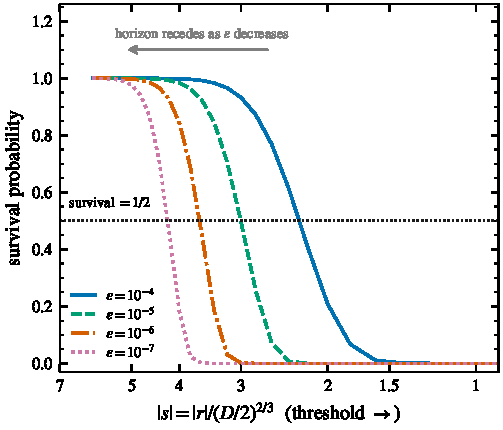
\includegraphics[width=\linewidth]{fig_horizon.pdf}
\caption{\label{fig:horizon}%
Survival along the ramp from Eq.~(\ref{eq:hazard}) at $D=0.09$.  The horizon recedes from threshold as $\varepsilon$ decreases, improving only as $[\ln(1/\varepsilon)]^{2/3}$.}
\end{figure}

%==============================================================================
\section{\label{sec:sat}What an observation carries}
%==============================================================================

We now return to the first of the two questions posed in Sec.~\ref{sec:intro}, and are careful to say which observation each answer is about.

\subsection{The snapshot information stays bounded, and peaks away from threshold}

Because the support of $\rho(\cdot\,;s)$ is independent of $s$ (Sec.~\ref{sec:law}), the family is regular and the Fisher information
\begin{equation}
\label{eq:Idef}
\Ifish_s(s)=\int\frac{(\partial_s\rho)^2}{\rho}\,\dd y
\end{equation}
exists, is finite, and is independent of sampling resolution.  It does not diverge.  It does something more interesting: it \emph{peaks and then declines}.
\begin{equation}
\label{eq:plateau}
\max_s\Ifish_s(s)=0.5425\ \text{at}\ s=-0.88,
\qquad
\Ifish_s(0)=0.4875(1),
\end{equation}
so the most informative snapshot of a ramped fold is not taken at threshold but roughly one noise scale away, at $|r|\simeq0.88\,(D/2)^{2/3}$, and approaching more closely makes a snapshot \emph{worse} --- by $10\%$ between the peak and $s=0$.  The maximum is flat, so its location is determined only to about $\pm0.05$; its height and the size of the decline are not.  In scaled terms $\Ifish_r(0)=0.4875(1)\,(D/2)^{-4/3}$, and the fitted log--log slope over $|s|\le0.25$ is $+0.013$, consistent with a finite limit rather than a residual power law.

By Lemma~\ref{thm:scaling} the whole profile is universal, so we tabulate it once (Table~\ref{tab:profile}) rather than leaving it only in Fig.~\ref{fig:info}.
\begin{table}[b]
\caption{\label{tab:profile}%
The universal snapshot information $\Ifish_s(s)$ of the conditioned law, against the OU surrogate $\Ifish^{\mathrm{OU}}$.  Any $(r,D)$ follows from $\Ifish_r=(D/2)^{-4/3}\Ifish_s(r/(D/2)^{2/3})$.  The ratio crosses unity at $|s|=1.24$ and stays below it thereafter: the surrogate is not uniformly an overestimate.}
\begin{ruledtabular}
\begin{tabular}{rccc}
\hline
$s$ & $\Ifish_s(s)$ & $\Ifish^{\mathrm{OU}}$ & ratio \\
\hline
$0$      & $0.48752$ & --- & --- \\
$-0.25$  & $0.51227$ & $3.00000$ & $5.86$ \\
$-0.50$  & $0.53094$ & $1.20711$ & $2.27$ \\
$-0.75$  & $0.54120$ & $0.79957$ & $1.48$ \\
$-0.88$  & $0.54258$ & $0.69442$ & $1.28$ \\
$-1.00$  & $0.54123$ & $0.62500$ & $1.15$ \\
$-1.50$  & $0.50918$ & $0.46380$ & $0.91$ \\
$-2.00$  & $0.44764$ & $0.38480$ & $0.86$ \\
$-3.00$  & $0.33227$ & $0.30256$ & $0.91$ \\
$-4.00$  & $0.27036$ & $0.25781$ & $0.95$ \\
$-8.00$  & $0.18099$ & $0.17873$ & $0.99$ \\
\end{tabular}
\end{ruledtabular}
\end{table}
One feature of the last column of Table~\ref{tab:profile} is worth noting, since it is easy to assume otherwise: the surrogate is not uniformly an overestimate.  The ratio $\Ifish^{\mathrm{OU}}/\Ifish_s$ crosses unity at $|s|=1.24$ and stays \emph{below} it from there outward, reaching a minimum of $0.86$ near $|s|=2$ --- OU understates the available information by up to $14\%$ --- and then returning to $1$ from below as the linearization becomes exact ($0.95$ at $|s|=4$, $0.99$ at $|s|=8$).  The failure of the linearization near a fold is therefore two-sided, and only inside $|s|\simeq1.24$ does it become the large one-sided overestimate that Sec.~\ref{sec:sat}\,C is about.

The non-monotonicity sharpens the paper's thesis rather than complicating it.  Critical slowing down is usually read as making a system progressively easier to interrogate as threshold approaches.  For the conditioned law it does not merely stop helping; past $|s|\simeq0.9$ it actively hurts, because the flux tail grows and drains probability out of the region where the density responds to $s$.  The saturation value $\Ifish_s(0)$ remains the right constant for the $D^{-4/3}$ scaling law and for the comparison with the surrogate, but it is a limit approached \emph{from above}, not a ceiling approached from below.

Deep in the well the exact information reproduces the surrogate~(\ref{eq:iou}), $\Ifish^{\mathrm{OU}}/\Ifish_s=0.99$ and $0.95$ at $s=-8$ and $-4$.  This is an important check: it confirms that the machinery is computing the same quantity the surrogate estimates, and that the discrepancy appearing at small $|s|$ is physical rather than numerical.

The OU divergence is therefore rounded off at the noise scale.  Quantitatively, the surrogate overstates the exact information by a factor of two only for
\begin{equation}
\label{eq:s2x}
|s|\lesssim0.61,\qquad\text{i.e.}\qquad |r|\lesssim0.077\ (D=0.09).
\end{equation}

\subsection{\label{sec:pathinfo}What that boundedness does not say}

Equation~(\ref{eq:plateau}) is a statement about \emph{one} draw from the conditioned law.  It is tempting --- and would be wrong --- to read it as a bound on how well the location of the fold can ever be learned.  We state the correct version because the incorrect one is the more quotable.

Let the observer see a continuous record of Eq.~(\ref{eq:fold}) with the fold location $\theta$ unknown, entering the drift as $r+\theta+x^2$.  The derivative of the drift with respect to $\theta$ is identically $1$, so Girsanov's theorem~\cite{LiptserShiryaev2001} gives the score as $U=D^{-1/2}\!\int_0^{\tau}\dd W$, a martingale, and optional stopping yields the path information
\begin{equation}
\label{eq:ipath}
\Ifish_{\mathrm{path}}=\frac{E[\tau]}{D},
\end{equation}
with $\tau$ the escape time.  Three facts follow, all verified numerically in Sec.~\ref{sec:num}.

First, Eq.~(\ref{eq:ipath}) grows without bound as observation continues --- it is the \emph{information}, not the escape time, that is unbounded --- so nothing saturates.  Second, the rate is exactly $1/D$ per unit \emph{surviving} time, uniformly in distance to the fold: measured window by window from $|s|=2.5$ to $|s|=0$, the ratio of the accumulated score variance to $E[t]/D$ stays within $1.3\%$ of unity, with no trend.  Approaching a saddle-node does not raise the information rate at all.  What falls near the fold is the expected remaining observation time, so proximity to the bifurcation is informationally neutral per unit time and strictly negative in total.  Third, the bound is attainable by a realistic discrete sampler: an Euler maximum-likelihood estimator reaches within $7\%$ of Eq.~(\ref{eq:ipath}) for sampling intervals up to $\Delta=0.1$, the residual excess being conditioning on non-escape rather than superefficiency, and degrading only at coarse spacing where Euler bias enters.

The reconciliation with Eq.~(\ref{eq:plateau}) is the point.  Critical slowing down makes a single snapshot sharper \emph{and} lengthens the correlation time over which snapshots repeat, and per unit time these compensate.  It is tempting to display that compensation by counting snapshots --- one per correlation time $1/(\mathrm{gap}\times\ell)$ gives $\Ifish_r(0)\times\mathrm{gap}\times\ell=1.93/D$, flat in $|r|$, against the exact $1/D$ of Eq.~(\ref{eq:ipath}) --- but a residual factor of two then has to be explained away as a sample-counting convention, and the explanation is not needed.  The comparison can be made exactly instead.

\emph{Which channel carries the spurious divergence.}  Apply Girsanov to the surrogate itself rather than to a count of snapshots.  Written as a diffusion in $x$ with $r$ the unknown, the OU surrogate has drift $b(x;r)=-2\sqrt{|r|}\,x+2r$, so $\partial_r b=x/\sqrt{|r|}+2$ and the information in a continuous record of length $T$ is $\Ifish^{\mathrm{OU}}(T)=(T/D)\,\mathbb{E}[(\partial_r b)^2]$ exactly.  Under the surrogate's own stationary law $x$ has mean $-\sqrt{|r|}$ and variance $D/(4\sqrt{|r|})$, so $\mathbb{E}[\partial_r b]=1$ and $\mathrm{Var}(\partial_r b)=D/(4|r|^{3/2})$, whence
\begin{equation}
\label{eq:channels}
\Ifish^{\mathrm{OU}}(T)
=\underbrace{\frac{T}{D}}_{\text{mean}}
+\underbrace{\frac{T}{4|r|^{3/2}}}_{\text{variance}} .
\end{equation}
No effective sample size enters.  The mean channel reproduces the exact path bound~(\ref{eq:ipath}) \emph{identically}, and it is the variance channel, alone, that diverges.  The OU surrogate is therefore not uniformly wrong near threshold: its mean channel is exact, and everything the conditioned law corrects sits in the term built from the variance.  That is worth stating plainly, because variance is the indicator early-warning practice actually computes, and Eq.~(\ref{eq:channels}) says the divergence it inherits is an artifact of the linearization rather than a property of the process.

That is not an abstract concern.  Masuda~\cite{Masuda2026} estimates the location of a bifurcation from the sample variance alone, fitting the power-law divergence the surrogate predicts, and reports estimates whose accuracy varies substantially across dynamical systems.  Equation~(\ref{eq:channels}) identifies the variance term as the one carrying the surrogate's entire spurious divergence, so a method reading the fold location out of that term is reading it out of the channel where the linearization is worst.  We do not claim this explains the reported variability, which its author attributes in part to the choice of tolerance band, and the comparison is not direct: that protocol equilibrates at each fixed control-parameter value rather than ramping continuously, so it has no $\Sig$ and the horizon~(\ref{eq:horizon_r}) does not apply to it as written.  What Eq.~(\ref{eq:channels}) does supply is the reason such methods should be expected to inherit a bias near threshold, and the scale $|r|\sim D^{2/3}$ at which it becomes order unity.

Equation~(\ref{eq:channels}) also disposes of the factor quoted above.  Matching it term by term against Eq.~(\ref{eq:iou}) requires $T\sqrt{|r|}$ effectively independent samples in the mean channel but $2T\sqrt{|r|}$ in the variance channel, because $x^2$ decorrelates at twice the rate of $x$.  A single effective sample size cannot serve both channels, which is why we do not use one; the apparent factor $1.9$ is that convention and carries no physical content.

The boundedness says that a single snapshot stops improving, and Sec.~\ref{sec:sat}\,A says it eventually gets worse.  Neither says that an observer stops improving, because an observer takes snapshots at a rate.

The operative limit at a noisy saddle-node is therefore not information-theoretic under a known model.  It is a limit on the \emph{states that occur} --- which is what the horizon of Sec.~\ref{sec:horizon} measures --- and, beyond the scope of this paper, on not knowing that the drift is $r+x^2$ in the first place.

\subsection{The regime where the surrogate fails is not observed}

Equations~(\ref{eq:horizon_s}) and~(\ref{eq:s2x}) can now be compared.  The most permissive ramp rate consistent with the quasi-static description in Table~\ref{tab:horizon} still has its horizon at $|s_h|=1.42$, more than twice $|s|_{2\times}=0.611$; slower ramps move the horizon further away still.  Across five decades of $\varepsilon$ the surrogate is accurate to between $4\%$ and $14\%$ at the horizon.

\emph{Over the rates that matter in practice, the regime in which the surrogate fails is not reached.}  Figure~\ref{fig:info} states this graphically: the shaded region contains the region where OU errs by a factor of two.

The containment has a domain, and stating it correctly turns out to matter more than asserting the containment.  Inverting the closed form~(\ref{eq:horizon_s}) to find where the \emph{quasi-static} median horizon meets $|s|_{2\times}$ gives $0.122$, but that is the wrong instrument for the question.  The claim is about where trajectories actually go, and Eq.~(\ref{eq:horizon_s}) is quasi-static: it omits the adiabatic lag $\tau_{\mathrm{eff}}\Sig$ that Sec.~\ref{sec:lag} derives and Sec.~\ref{sec:num} measures.  At the rates of Table~\ref{tab:horizon} that lag is a $2\%$ correction and can be ignored; at $\Sig=0.122$ it is $\tau_{\mathrm{eff}}\Sig=0.139$, which is $23\%$ of the horizon it is being applied to.  Direct Euler--Maruyama integration of Eq.~(\ref{eq:fold}) gives the medians in Table~\ref{tab:containment}.
\begin{table}[b]
\caption{\label{tab:containment}%
Median escape location at ramp rates near the containment threshold, in scaled units, against $|s|_{2\times}=0.611$.  ``Closed form'' is Eq.~(\ref{eq:horizon_s}); ``exact q.s.'' replaces the Kramers rate by the exact eigenvalue but is still quasi-static; ``simulated'' is direct Euler--Maruyama integration of Eq.~(\ref{eq:fold}) and is the only column that carries the adiabatic lag.  Errors are batch standard errors on the last digit.}
\begin{ruledtabular}
\begin{tabular}{lccc}
\hline
$\Sig$ & closed form & exact q.s. & simulated \\
\hline
$0.080$ & $0.855$ & $0.830$ & $0.748(4)$ \\
$0.100$ & $0.730$ & $0.715$ & $0.611(3)$ \\
$0.122$ & $0.608$ & $0.609$ & $0.487(5)$ \\
$0.150$ & $0.467$ & $0.495$ & $0.338(4)$ \\
\end{tabular}
\end{ruledtabular}
\end{table}
At $\Sig=0.122$ the median trajectory reaches $|s|=0.487$, well \emph{inside} the region where the surrogate errs by a factor of two, and $58\%$ of the ensemble survives to $|s|_{2\times}$.  The correct threshold is
\begin{equation}
\label{eq:sigcont}
\Sig_{\mathrm{cont}}\simeq0.10 ,
\end{equation}
which we quote to two digits because at these rates the $O(\Sig)$ lag expansion is itself a $20\%$ correction and a third digit would not be meaningful.  Three independent checks agree: the simulated median horizon at $\Sig=0.100$ is $0.611(3)$, equal to $|s|_{2\times}$; the surviving fraction at $|s|_{2\times}$ is then $0.501$, one half, as the definition requires; and inverting the first-order lag correction analytically, $|s_h|^{\mathrm{q.s.}}(\Sig)-\tau_{\mathrm{eff}}\Sig=|s|_{2\times}$, gives $0.10$.

Two features of the table are worth drawing out.  The Kramers prefactor is \emph{not} the culprit: at $\Sig=0.122$ the closed form ($0.608$) and the exact-eigenvalue quasi-static horizon ($0.609$) agree to $0.15\%$, because the prefactor's overestimate at moderate barrier and its underestimate at small barrier cancel near $|s|\simeq0.9$ (Appendix~\ref{app:kramers}).  The entire discrepancy is the lag.  And the corrected threshold is consistent with Ref.~\cite{HerbertBouchet2017}, which reports its adiabatic description becoming accurate only above $\epsilon_{\mathrm{HB}}\approx20$: by Eq.~(\ref{eq:dictionary}) that is $\Sig\lesssim0.05$, whereas $\Sig=0.122$ corresponds to $\epsilon_{\mathrm{HB}}=8.2$ --- inside the range that reference explicitly flags.

Three distinct ramp-rate thresholds appear in this paper and are easily confused, so we collect them once:
\begin{table}[b]
\caption{\label{tab:thresholds}%
The three ramp-rate limits, in increasing order.  Each answers a different question, and the binding one is the smallest.  Every rate in Table~\ref{tab:horizon} satisfies all three.}
\begin{ruledtabular}
\begin{tabular}{llll}
$\Sig$ & name & what fails above it & from \\
\hline
$0.10$  & containment & the median trajectory enters & Eq.~(\ref{eq:sigcont}) \\
        &             & the surrogate's failure region & \\
$0.201$ & adiabaticity & the quasi-static reading of & Sec.~\ref{sec:kz} \\
        &              & the hazard is no longer safe & \\
$0.230$ & domain & the closed form is undefined; & Eq.~(\ref{eq:domain}) \\
        &        & the ramp outruns escape & \\
\end{tabular}
\end{ruledtabular}
\end{table}
The ordering is the useful content.  Containment is the strictest, so an analysis that checks only Eq.~(\ref{eq:domain}) --- the condition under which the formula returns a number at all --- can be a factor $2.3$ inside the regime where that number describes a trajectory the ensemble actually follows.

Every rate in Table~\ref{tab:horizon} lies below Eq.~(\ref{eq:sigcont}) by a factor of at least $4.5$, so the containment claim survives intact where the paper actually applies it.  But the closed form's own domain~(\ref{eq:domain}) extends to $\Sig<0.230$, so there is an interval --- a factor $2.3$ wide --- in which Eq.~(\ref{eq:horizon_r}) is perfectly well defined and the median horizon nonetheless lies inside the failure region.  At $\Sig=0.15$, $66\%$ of the ensemble survives to $|s|_{2\times}$.  We therefore do not claim containment across the whole domain of the closed form, and Fig.~\ref{fig:info} should be read as describing $\Sig<0.10$.

Within that range two conventions still have to be varied --- the horizon depends on the survival level defining it, the threshold on the factor at which the surrogate is called wrong --- and the containment survives both, though only for typical trajectories.  Over the rates of Table~\ref{tab:horizon} and survival levels $P\in[0.1,0.9]$ the smallest quasi-static horizon is $|s_h|=0.898$, which the lag of Sec.~\ref{sec:lag} reduces to $0.873$ --- the correction must be applied here too, for the reason this subsection has just given --- and containment then holds for every $f>1.43$, where $|s|_f$ is defined by $\Ifish^{\mathrm{OU}}=f\,\Ifish_s(0)$; that critical factor moves by less than $1\%$ across the quoted uncertainty in $\Ifish_s(0)$.  At the faster rate $\Sig=0.05$ used in Sec.~\ref{sec:stommel} the tenth-percentile horizon falls to $0.389$, inside $|s|_{2\times}$, and direct integration of Eq.~(\ref{eq:fold}) gives a survival probability of $0.217$ at $|s|=0.61$.  A fifth of that ensemble does reach the region in which the surrogate is wrong.

One convention runs the other way and we record it, since it makes the failure region smaller than drawn.  Defining $|s|_f$ against the plateau $\Ifish_s(0)$ compares the surrogate with the information available at threshold rather than with the exact information at the same $s$.  The latter is the more natural criterion, and because $\Ifish_s(s)$ exceeds its threshold value over the whole relevant range (Sec.~\ref{sec:sat}\,A), it places the two-fold crossing at $|s|=0.56$ rather than $0.61$.  We keep the conservative $0.61$ throughout, so every containment margin quoted here is an underestimate.

This resolves the two questions together, and neither answer alone would have been informative.  The divergence is \emph{not} real --- the exact snapshot information stays bounded.  And for $\Sig\lesssim0.10$ the failure of the surrogate is not observed by a typical trajectory, because it lives inside the region the bulk of the ensemble has already vacated.  A practitioner using OU near a slowly ramped fold is therefore making a defensible approximation, not because the approximation is exact, but because its error is confined to states that a typical realization does not occupy.

\begin{figure}[t]
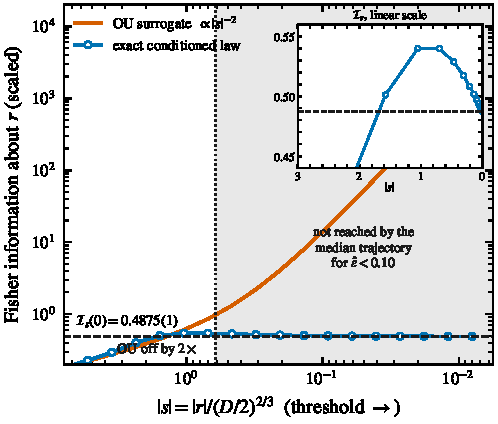
\includegraphics[width=\linewidth]{fig_information.pdf}
\caption{\label{fig:info}%
Per-observation Fisher information about $r$.  The OU surrogate diverges as $|s|^{-2}$; the exact conditioned law does not, peaking at $0.5425$ near $s=-0.88$ and declining to $\Ifish_s(0)=0.4875(1)$ at threshold.  Shading marks the region that the median trajectory does not reach at any ramp rate $\Sig<0.10$; its boundary \emph{is} $|s|_{2\times}$ (dotted), where the surrogate first errs by a factor of two against the plateau, since $\Sig_{\mathrm{cont}}$ is defined by the coincidence of the two.}
\end{figure}

\subsection{\label{sec:census}Coarse-graining the tipping record: an exact result, and not a fold result}

The escape law that closes the window is itself an observation, and it is a good one.  This subsection quantifies it, and extracts from it a design rule that requires no knowledge of $D$, $\varepsilon$ or the barrier height.

Write $w=\tfrac43\sigma^{3/2}$ with $\sigma\equiv|s|$, and $\mu=\ln[1/(2\pi\,\Sig)]$.  Equation~(\ref{eq:hazard}) then says that the survival function is
\begin{equation}
\label{eq:gumbel}
S=\exp\bigl[-e^{-(w-\mu)}\bigr],
\end{equation}
that is, the tipping law is \emph{exactly} standard Gumbel in $w$, with unit scale~\cite{Gumbel1958}.

\emph{The generality of what follows, stated before the result.}  It would be easy to present the rest of this subsection as a consequence of that exact integrability.  It is not one, and we say so at the outset because the temptation to overclaim here is strong.  Let $\hat H$ be \emph{any} strictly increasing cumulative hazard and let the unknown be its log-scale, $H=e^{\theta}\hat H$.  Then $u=e^{\theta}\hat H(\text{escape})$ is $\mathrm{Exp}(1)$ by the probability-integral transform, so $\partial_\theta\ln f=1-u$ and
\begin{equation}
\label{eq:ftau}
F_\tau=\mathbb{E}\bigl[(1-u)^2\bigr]=\mathrm{Var}(u)=1
\end{equation}
exactly, while one tipped/not-tipped census at $u$ carries
\begin{equation}
\label{eq:fbin}
F_{\mathrm{bin}}(u)=\frac{(\partial_\theta p)^2}{p(1-p)}=\frac{u^2}{e^{u}-1}\equiv g(u),
\end{equation}
verified against a central difference of $p$ to $10^{-10}$ relative.  Neither expression contains the fold, the $|s|^{3/2}$ barrier, Kramers' formula, or the integrability of Eq.~(\ref{eq:hazard}); we confirmed by direct simulation that a Weibull hazard $\hat H\propto x^3$, a log-logistic hazard and a strongly oscillatory one all return the same constants to seven digits.  This is a quantal-response/type-I-censoring fact about proportional-hazards families, and the optimal placement of a single censoring time for an extreme-value law is classical design theory~\cite{Gertsbakh1995,LehmannCasella1998}.  We include it because it is useful for the systems this paper is about and appears not to be known in the tipping literature, not because it is new statistics or a property of the saddle-node.

\emph{Which parameter.}  Equations~(\ref{eq:ftau})--(\ref{eq:fbin}) concern $\theta$, the log-scale of the hazard --- for the ramped fold, the combination $\mu=\ln[1/(2\pi\,\Sig)]$ of ramp rate and noise.  That is \emph{not} the location of the fold, and the design rule below should not be read as one for locating a bifurcation; Sec.~\ref{sec:sat}\,E treats that parameter separately and reaches a different optimum.

\emph{Two universal constants.}  Maximizing $g$ gives $2(e^u-1)=u e^u$, hence
\begin{equation}
\label{eq:ustar}
u^\ast=1.5936243,\qquad g(u^\ast)=0.6476102 .
\end{equation}
A single yes/no observation therefore recovers $64.8\%$ of the information in the full tipping-time record.  Timing individual tippings is worth a factor $1.54$, not a change of scaling.  The optimum sits at survival $e^{-u^\ast}=0.203188$:

\begin{quote}
\emph{The optimal census is taken when $79.68\%$ of the ensemble has tipped.}
\end{quote}

\noindent This is parameter-free --- independent of $\Sig$, $D$, ramp rate and barrier height, and, by the argument above, of the hazard shape.  It is also self-referential: the observer reads the stopping condition off the tipped fraction itself and needs no prior estimate of $\mu$, which is what makes it an operational prescription rather than an oracle result.  The prescription is forgiving: at least $90\%$ of the maximum is retained for tipped fractions anywhere in $[0.633,0.904]$, at least $95\%$ in $[0.688,0.878]$, and at least $99\%$ in $[0.752,0.836]$.

\emph{More censuses nest upward.}  With $m$ censuses the observation is a multinomial over $m+1$ bins.  Optimizing the placement (Nelder--Mead, $80$ restarts) gives efficiencies
\begin{equation}
\label{eq:nesting}
\begin{aligned}
&0.6476,\ 0.8203,\ 0.8910,\ 0.9269,\\
&0.9476,\ 0.9606,\ 0.9754,\ 0.9832
\end{aligned}
\end{equation}
for $m=1,2,3,4,5,6,8,10$: monotone toward $1$, as it must be, since the tipped indicator observed at every $w$ \emph{is} the tipping time.  These too are exact pure numbers, independent of $\Sig$.  The optimal five-point design sits at tipped fractions $0.393$, $0.667$, $0.843$, $0.943$, $0.988$.  The deficit $1-F_m$ falls slightly more slowly than $1/m^2$, empirically as ${\approx}0.8\ln m/m^2$; we state that as a fit, not a derivation.

\emph{The bound is attained.}  A maximum-likelihood estimator~\cite{LehmannCasella1998} from $N$ binary observations at $u^\ast$ has a variance-to-Cram\'er--Rao-bound ratio $\mathrm{Var}/\mathrm{CRB}=1.041$, $1.002$, $0.988$, $0.975$ at $N=200$, $10^3$, $5\times10^3$, $2\times10^4$.  Individually each deviation is within Monte Carlo scatter --- on $4000$ replicates the relative standard error of a variance estimate is $\sqrt{2/4000}=2.2\%$ --- but the sequence is monotone, which scatter alone does not produce, so we state the weaker conclusion the data support: the ratio approaches unity from above and settles within $2.5\%$ below it, consistent with attainment but not establishing it to better than a few percent.  A definitive statement would need more replicates than we have run.

Two limitations bound what this subsection claims.  The channel requires an ensemble --- $N$ realizations give $N F_{\mathrm{bin}}$ --- so it speaks to repeated or spatially replicated systems, not to a single time series.  And attainability has been established for the binary channel only; the corresponding statement for an estimator built from observed tipping times is not tested.

\subsection{\label{sec:foldloc}The same question for the fold location}

The parameter of Sec.~\ref{sec:sat}\,D is the hazard scale.  An observer who wants the \emph{position} of the bifurcation is asking a different question, and the answer differs in a way worth recording, not least because the obvious shortcut fails.

Let the fold sit at $s=\theta$ with $\theta$ unknown, so that every quantity depends on $s-\theta$.  Along the ramp the escape density in $s$ is $f(s)=\tilde\lambda(s)P(s)/\Sig$ with $P=\exp[-\Sig^{-1}\!\int^s\tilde\lambda]$, and the score is $-\dd\ln f/\dd s=\tilde\lambda/\Sig-\tilde\lambda'/\tilde\lambda$.

If one inserts the Kramers rate~(\ref{eq:kramers}) here, its $\sqrt{|s|}$ prefactor vanishes at threshold, the term $\tilde\lambda'/\tilde\lambda$ acquires a $1/2s$ pole, and the Fisher information \emph{diverges}: the integrand behaves as $|s|^{-3/2}$ and the value grows without bound as the cutoff at the fold is lowered.  It would be easy to report that divergence as a second instance of the non-regularity Sec.~\ref{sec:law}\,B rejects.  That would be wrong.  The exact rate does not vanish at threshold --- $\tilde\lambda(0)=0.35412$, continuing smoothly past it to $\tilde\lambda(0.5)=0.610$ and $\tilde\lambda(1)=0.962$ --- and with the exact rate the information is finite and cutoff-free.  Continuing the model to $s=+0.5$, $+1$ and $+2$ gives $F_{\mathrm{fold}}=4.6940$, $4.6939$, $4.6939$ at $\Sig=2.22\times10^{-2}$: insensitive to the continuation at the fourth decimal.  \emph{The non-regularity is a property of the approximation, not of the problem}, and this is the one place where the Kramers form must be given up rather than merely corrected.

With the exact rate, the census result survives in part and fails in part.  The efficiency of a single binary census is essentially unchanged --- $F_{\mathrm{bin}}/F_{\mathrm{fold}}=0.649$, $0.647$, $0.645$ at $\Sig=2.22\times10^{-2}$, $0.05$, $0.10$, still within a percent of $g(u^\ast)$ --- but the optimal \emph{placement} moves:
\begin{equation}
\label{eq:foldopt}
\text{tipped fraction at the optimum}=0.700,\ 0.678,\ 0.657
\end{equation}
at those three rates, against $0.7968$ for the hazard scale.

\emph{How the fold-location information scales.}  The three values above sit on a scaling law that follows from machinery already in the paper.  With the Kramers rate and the exact integrability of Sec.~\ref{sec:horizon}\,B, $\dd\ln\lambda/\dd s=2\sqrt\sigma-1/2\sigma$ and $\lambda/\Sig=2\sqrt\sigma\,u$ with $u\sim\mathrm{Exp}(1)$, so the score for the fold location is
\begin{equation}
\label{eq:foldscore}
\partial_\theta\ln f=2\sqrt\sigma\,(1-u)-\frac{1}{2\sigma},
\end{equation}
and, since $\E[(1-u)^2]=1$ and the cross term vanishes, $F_{\mathrm{fold}}\simeq4\sigma+1/4\sigma^2$ with $\sigma$ evaluated at the horizon.  The leading term is $4|s_h|$.  Computing $F_{\mathrm{fold}}$ with the exact rate over two decades gives $F_{\mathrm{fold}}/4|s_h|=0.840$, $0.807$, $0.833$, $0.855$, $0.875$ at $\Sig=0.05$, $2.22\times10^{-2}$, $5\times10^{-3}$, $2.22\times10^{-3}$, $10^{-3}$: the ratio approaches unity from below, but slowly, the residual being the variation of $\sqrt\sigma$ across the Gumbel spread.  We therefore state $4|s_h|$ as the asymptotic form and not as a converged number.

This closes the paper's information ledger.  A snapshot carries at most $\Ifish_s(0)(D/2)^{-4/3}$; a continuous record carries $1/D$ per unit surviving time; a tipping time carries $\simeq4|s_h|$.  Every channel closes logarithmically in the ramp rate, because $|s_h|\sim[\ln(1/\varepsilon)]^{2/3}$ is the only place $\varepsilon$ enters.  The practical form of that statement is the least encouraging one: since the standard error on the fold location falls as $F_{\mathrm{fold}}^{-1/2}\sim[\ln(1/\varepsilon)]^{-1/3}$, halving it requires raising $\varepsilon$ to the eighth power.  An observer whose target is the bifurcation point should census earlier than one whose target is the escape rate, and unlike Eq.~(\ref{eq:ustar}) this optimum is not universal: it drifts with the ramp rate, because $\tilde\lambda$ has no scale invariance that $\mu$ can absorb.

%==============================================================================
\section{\label{sec:lag}Adiabatic validity and the first-order correction}
%==============================================================================

Every statement in Sec.~\ref{sec:horizon} presupposes that the conditioned law relaxes faster than $r$ changes.  This section establishes when that holds, shows that the regime in which it fails is never entered, and computes the leading correction.

\subsection{The validity condition}

Relaxation of the conditioned law proceeds at the spectral gap of Eq.~(\ref{eq:killed}), measured as $1.82$--$1.95$ over $s\in[-2,-0.25]$, i.e.\ at rate $\ell\times O(1)$.  An $O(1)$ change in $s$ takes time $\ell^2/\varepsilon$.  The quasi-static description therefore requires
\begin{equation}
\label{eq:adiabatic}
\varepsilon\ll D/2,
\end{equation}
satisfied by factors of $45$ to $4.5\times10^{5}$ for the rates in Table~\ref{tab:horizon}.  Faster ramps enter the rate-induced regime~\cite{Ashwin2012,Ritchie2016,Alkhayuon2019}, in which the frozen-$r$ law is not the correct description at all and the present analysis does not apply.

\subsection{\label{sec:kz}The non-adiabatic regime is never entered}

Equation~(\ref{eq:adiabatic}) bounds the size of the correction.  A stronger statement is available: the regime it excludes cannot be reached, because escape destroys the ensemble first.

The Kibble--Zurek construction~\cite{Kibble1976,Zurek1985,delCampoZurek2014} locates freeze-out where the relaxation time equals the time remaining to the transition.  Here $\tau_{\mathrm{relax}}=1/(2\sqrt\sigma)$ and the time remaining is $\sigma/\Sig$, so freeze-out sits at $\sigma_{\mathrm{KZ}}=(\Sig/2)^{2/3}$.  Both this and the horizon $|s_h|$ of Eq.~(\ref{eq:horizon_s}) are scaled quantities, and their ratio is therefore independent of $D$:
\begin{equation}
\label{eq:kzratio}
\frac{|s_h|}{\sigma_{\mathrm{KZ}}}
=\Bigl[\frac{\tfrac32\ln\bigl(1/2\pi\ln2\,\Sig\bigr)}{\Sig}\Bigr]^{2/3}
\longrightarrow\infty
\qquad(\Sig\to0),
\end{equation}
a logarithm over a power.  The ratio is $29$, $214$, $1.3\times10^3$, $7.3\times10^3$ and $3.9\times10^4$ for $\Sig=2.22\times10^{-2}$ down to $2.22\times10^{-6}$.  The ensemble is destroyed by activated escape long before the ramp outruns relaxation, by a margin that grows without bound as the ramp slows, so the quasi-static hazard is self-consistent for a stated reason and not by assumption.

The statement has a boundary, and it is worth being exact about where.  Solving $|s_h|=\sigma_{\mathrm{KZ}}$ gives a crossover at $\Sig=0.201$; above that, freeze-out precedes the horizon and the quasi-static description fails before escape has removed half the ensemble.  That crossover lies \emph{inside} the domain~(\ref{eq:domain}) of the closed form, $\Sig<0.230$, not outside it.  The argument of this subsection therefore covers $\Sig<0.201$ --- every rate in Table~\ref{tab:horizon} by a factor of at least nine --- but not the last narrow sliver of the permitted domain, where Eq.~(\ref{eq:horizon_r}) is still defined and the adiabatic reading of it is no longer safe.

Two consequences are worth recording.  \emph{Kibble--Zurek scaling is never observable at a noisy saddle-node}: an experiment fitting KZ exponents there is measuring escape statistics instead.  This is falsifiable and worth stating, because KZ exponents are fitted routinely in the quench literature.  And the two $2/3$ exponents in this paper are unrelated physics that happen to coincide: $\Sig^{2/3}$ is the deterministic sweep scaling, $[D\ln(1/\varepsilon)]^{2/3}$ is activated escape.  They look identical and should not be conflated.  We note that this monotone-ramp conclusion does not contradict Refs.~\cite{DykmanGoldingRyvkine2004,RyvkineDykmanGolding2004}, where adiabaticity does break down near the bifurcation: there the drive is periodic and the system revisits the critical region indefinitely, so the escape that ends the approach here never gets the chance to occur.

\subsection{The correction is exact at first order}

Write $\nu=N(\tau)\bigl[\rho(s)+\Sig\,\rho_1(s)+\cdots\bigr]$ with $\int\rho_1=0$ and $\dd\ln N/\dd\tau=-\lambda-\Sig\,\mu_1$.  Matching at $O(\Sig)$ gives $(\Leff^\ast+\lambda)\rho_1=\partial_s\rho-\mu_1\rho$.  The operator on the left is singular, and Fredholm solvability against the left eigenfunction $\phi$ (defined by $\Leff\phi=-\lambda\phi$, $\langle\phi,\rho\rangle=1$) yields the correction in closed form:
\begin{equation}
\label{eq:mu1}
\mu_1(s)=\langle\phi,\partial_s\rho\rangle,
\qquad
\ln\frac{P}{P_{\mathrm{ad}}}=-\int\mu_1\,\dd s' .
\end{equation}
The derivation is given in full in Appendix~\ref{app:lag}.

\subsection{An independent check of the adjoint machinery}

Equation~(\ref{eq:mu1}) involves the left eigenfunction, which is not directly observable, so an independent validation is valuable.  Since $\partial_s\Leff=\partial_y$, the Hellmann--Feynman theorem gives
\begin{equation}
\label{eq:hf}
\lambda'(s)=-\langle\rho,\partial_y\phi\rangle,
\end{equation}
a relation between quantities computed by different routes.  It reproduces the numerically differentiated $\lambda'$ to better than $0.11\%$ over $s\in[-2,-0.1]$, confirming that $\phi$, the normalization $\langle\phi,\rho\rangle=1$, and the inner products are all correct.  The check has content only because $\phi$ is obtained here from the transposed operator with $\langle\phi,\rho\rangle=1$ imposed explicitly; in the symmetric conjugate representation the normalization is automatic and the identity cannot fail.

\subsection{Magnitude and empirical form}

Empirically $-\mu_1/\lambda'$ is close to constant, $1.11\pm0.08$ over $s\in[-2,-0.1]$, so the correction is well approximated by
\begin{equation}
\label{eq:taueff}
\ln\bigl(P/P_{\mathrm{ad}}\bigr)\simeq\tau_{\mathrm{eff}}\,\lambda(s),\qquad \tau_{\mathrm{eff}}\simeq1,
\end{equation}
which is notably \emph{independent} of the ramp rate, the explicit $\Sig$ having canceled.  Direct simulation gives $\tau_{\mathrm{eff}}=1.14\pm0.09$ across three ramp rates spanning a factor of ten, consistent within uncertainties with the eigenvalue determination $-\mu_1/\lambda'=1.11\pm0.08$.  In both determinations $\tau_{\mathrm{eff}}\times\text{gap}\approx2$.

We stress that Eq.~(\ref{eq:taueff}) is an approximation to the exact statement~(\ref{eq:mu1}); $-\mu_1/\lambda'$ drifts by about $21\%$ across the range quoted, and we do not claim it is constant.  The correction shifts the horizon by $\tau_{\mathrm{eff}}\,\Sig$, i.e.\ by $0.025$ in $|s_h|$ at $\varepsilon=10^{-3}$, and vanishes as $\varepsilon\to0$.  Section~\ref{sec:num} reports a quantitative test of this shift.

%==============================================================================
\section{\label{sec:stommel}Application: a two-box thermohaline model}
%==============================================================================

Everything so far concerns the normal form~(\ref{eq:fold}): one dimension, additive noise.  A physical system near a saddle-node is neither.  This section asks whether the closed form survives the reduction of a genuine multidimensional model --- and answers by predicting that model's collapse point with no fitted parameters.

\subsection{The model}

We use the Stommel two-box model of thermohaline circulation~\cite{Stommel1961,Cessi1994}, the standard minimal model for a bistable overturning flow and the ancestor of the box models used in current tipping-point studies~\cite{Alkhayuon2019,Ditlevsen2023}.  On the smooth branch $q\equiv T-S>0$,
\begin{equation}
\label{eq:stommel}
\begin{aligned}
\dot T&=\eta_1-T(1+q),\\
\dot S&=\eta_2-S(\eta_3+q)+\sigma\,\dot W,
\end{aligned}
\end{equation}
with $\eta_1=3$, $\eta_3=0.3$, and the freshwater forcing $\eta_2$ ramped toward the fold at rate $v$.  Two features make this a genuine test rather than a relabeling.  The system is two-dimensional, so the reduction to Eq.~(\ref{eq:fold}) must actually be performed.  And the noise acts \emph{only} on salinity, so the effective diffusion entering Eq.~(\ref{eq:horizon_r}) is a nontrivial projection of the applied noise rather than the applied variance itself.

\subsection{Locating the fold and reducing to the normal form}

Solving $F=0$ together with $\det\partial F/\partial X=0$ places the saddle-node at
\begin{equation}
\eta_2^c=1.220115317196,\qquad
\begin{aligned}
T_c&=2.155268505,\\ S_c&=1.763330567,
\end{aligned}
\end{equation}
with Jacobian eigenvalues $\{0,-2.4758\}$: a simple zero eigenvalue and a strongly contracting transverse direction, as a codimension-one saddle-node requires.

Let $e$ and $f$ be the right and left null vectors of the Jacobian, normalized by $f^{\mathsf T}e=1$.  Center-manifold reduction (Appendix~\ref{app:cmf}) gives $\dot z=a\,\delta\eta_2+b\,z^2$ with
\begin{equation}
\label{eq:ab}
a=f^{\mathsf T}\partial_{\eta_2}F,\qquad b=\tfrac12 f^{\mathsf T}D^2F[e,e],
\end{equation}
and the rescaling $x=bz$ carries this to the normal form~(\ref{eq:fold}) with
\begin{equation}
\label{eq:reduction}
r=P\,\delta\eta_2,\qquad P\equiv ab,\qquad
\boxed{\;D_{\mathrm{eff}}=b^2\,f^{\mathsf T}\Sigma\Sigma^{\mathsf T}f\;}
\end{equation}
and ramp rate $\varepsilon_{\mathrm{eff}}=Pv$.  For Eq.~(\ref{eq:stommel}) the vector field is quadratic, so $D^2F$ is constant and both coefficients are exact rather than numerical:
\begin{equation}
a=f_2,\qquad b=(e_2-e_1)(f_1e_1+f_2e_2),
\end{equation}
giving $a=-1.6764771290$, $b=-0.3353545916$, and $P=0.5622143030$.

Two internal consistency checks are worth recording.  The normalization of $e$ is arbitrary, and under $e\to ke$ one has $a\to a/k$, $b\to kb$; the physical outputs $P$ and $D_{\mathrm{eff}}$ must therefore be invariant, and they are, to ten digits.  And the reduced normal form must reproduce the true equilibrium branch of Eq.~(\ref{eq:stommel}); it does, to $0.04\%$ at $\delta\eta_2=-10^{-5}$, degrading as $\sqrt{|\delta\eta_2|}$ exactly as the neglected $O(z^3)$ term requires.

Because the noise enters only the second component, $D_{\mathrm{eff}}=(P\sigma)^2$.  An analysis that used the applied variance $\sigma^2$ in place of its projection would be wrong by a factor $P^2\approx0.32$ --- an error of the same order as the effect being measured.

\subsection{The prediction, and the test}

We now feed $D_{\mathrm{eff}}$ and $\varepsilon_{\mathrm{eff}}$ into Eq.~(\ref{eq:horizon_r}) and compare with direct simulation of the \emph{full two-dimensional} system~(\ref{eq:stommel}).  Nothing is fitted: $\sigma$ and $v$ are chosen to set $(D_{\mathrm{eff}},\Sig)$, and every other quantity follows from the fold location and two eigenvectors.  Table~\ref{tab:stommel} reports the result, together with a simulation of the reduced one-dimensional normal form under the same escape rule.

\begin{table}[b]
\caption{\label{tab:stommel}%
Observability horizon of the two-box model~(\ref{eq:stommel}) at $D_{\mathrm{eff}}=10^{-4}$.  ``Closed form'' is Eq.~(\ref{eq:horizon_s}) evaluated at $\Sig=2\varepsilon_{\mathrm{eff}}/D_{\mathrm{eff}}$ with no fitted parameters.  Uncertainties are standard errors over six independent batches of $3000$ paths.}
\begin{ruledtabular}
\begin{tabular}{lrrr}
$\Sig$ & closed form & reduced 1-D & full 2-D \\
\colrule
$0.050$ & $1.0934$ & $1.0026(33)$ & $1.0179(43)$ \\
$0.020$ & $1.4964$ & $1.4412(21)$ & $1.4550(24)$ \\
\end{tabular}
\end{ruledtabular}
\end{table}

In physical variables, at $\Sig=0.02$ the closed form predicts collapse at $\eta_2=1.216503$ and the two-dimensional simulation measures $\eta_2=1.216603$.  Figure~\ref{fig:stommel}(a) shows the full survival curves rather than only their midpoints: the closed form tracks the two-dimensional model over the entire transition, not merely at $P=\tfrac12$.

Figure~\ref{fig:stommel}(b) displays the same statement in the model's own variables.  The two-box system has a genuine fold at $\eta_2^c=1.2201$; the normal-form parabola obtained by reduction --- not by fitting --- follows the exact equilibrium branch through the region that matters; and the horizon falls at $\eta_2=1.2165$, a visible distance \emph{before} the fold.  The shaded interval --- the last $0.0036$ of the approach in $\eta_2$, equivalently the whole of $|s|<1.50$ --- is the part of the approach that a ramped ensemble does not survive to report on.

\begin{figure*}[t]
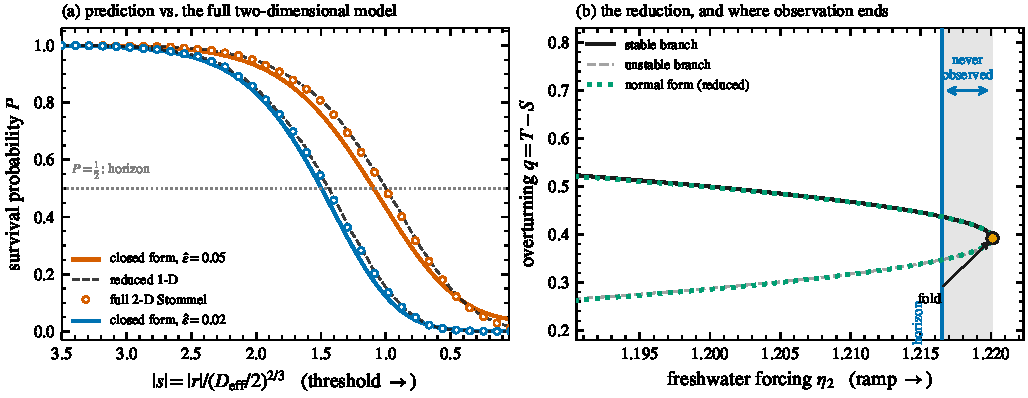
\includegraphics[width=\linewidth]{fig_stommel.pdf}
\caption{\label{fig:stommel}%
The two-box thermohaline model of Eq.~(\ref{eq:stommel}).
(a)~Survival along the ramp at two rates.  Solid curves are the closed form~(\ref{eq:hazard}) with no fitted parameters; dashed curves are the reduced 1-D normal form; open circles are direct simulation of the full two-dimensional system.  The dotted line marks $P=\tfrac12$, which defines the horizon.
(b)~The equilibrium branches of the two-box model in its own variables, with the fold at $\eta_2^c=1.2201$ and the normal-form parabola obtained by center-manifold reduction (dotted, green).  The observability horizon at $\Sig=0.02$ lies at $\eta_2=1.2165$; the shaded region between it and the fold is never observed, because the ensemble has escaped.}
\end{figure*}

\subsection{Where the error lives}

The comparison in Table~\ref{tab:stommel} is usually read as a two-way split, closed form against reduction.  That reading is wrong, and the number that corrects it is measured in Sec.~\ref{sec:num}.  ``Closed form'' is \emph{both} quasi-static \emph{and} Kramers, while the reduced one-dimensional column is a ramped simulation carrying the adiabatic lag of Sec.~\ref{sec:lag}.  Inserting the quasi-static eigenvalue horizon --- $1.0584$ and $1.4617$, the numbers already used for the lag test in Sec.~\ref{sec:num} --- as the missing intermediate reference splits the discrepancy three ways (Table~\ref{tab:errorsplit}, writing ``q.s.'' for quasi-static and ``cf'' for the closed form).
\begin{table}[b]
\caption{\label{tab:errorsplit}%
Three-way decomposition of the discrepancy in Table~\ref{tab:stommel}.  Each row is normalized to its own reference --- the Kramers term to the quasi-static horizon, the lag and reduction terms to the 1-D simulation, the net to the 2-D simulation --- so the rows do not sum.  The reduction term carries the opposite sign to the other two, which is what ``partially cancel'' means below.  At the faster ramp the adiabatic lag, not the Kramers prefactor, is the largest single contribution.}
\begin{ruledtabular}
\begin{tabular}{lcc}
\hline
source & $\Sig=0.05$ & $\Sig=0.02$ \\
\hline
Kramers (cf vs.\ q.s.)   & $3.3\%$ & $2.4\%$ \\
adiabatic lag (q.s.\ vs.\ 1-D) & $5.6\%$ & $1.4\%$ \\
reduction (1-D vs.\ 2-D) & $1.5\%$ & $1.0\%$ \\
\hline
net (cf vs.\ 2-D)        & $7.4\%$ & $2.8\%$ \\
\end{tabular}
\end{ruledtabular}
\end{table}
At $\Sig=0.05$ the \emph{adiabatic lag}, not the Kramers prefactor, is the largest single contribution; at $\Sig=0.02$ the Kramers term dominates.  This is the expected ordering --- the lag scales as $\tau_{\mathrm{eff}}\,\Sig$ and so falls linearly with the ramp rate, while the Kramers error falls only with barrier height --- and it turns Sec.~\ref{sec:lag} from a consistency argument into a correction that is doing visible work: expressed as fractions of the simulated horizon, $\tau_{\mathrm{eff}}\Sig$ predicts $5.7\%$ and $1.6\%$ against the $5.6\%$ and $1.4\%$ found here.  Reducing a genuine two-dimensional physical model to the normal form costs about one percent at both rates, and remains the smallest of the three.  The net figure is strongly rate-dependent, and we quote both rates wherever it is cited.

The measurement is robust to its numerical conventions: halving the time step changes $|s_h|$ by $1.7\%$, varying the escape threshold over $Y\in[5,12]$ by $0.6\%$, and starting the ramp earlier by $1.1\%$.  Throughout, $q$ remained positive (minimum $0.089$), so the smooth branch of Eq.~(\ref{eq:stommel}) was never violated.

\subsection{What this does and does not establish}

It establishes that Eq.~(\ref{eq:horizon_r}) is predictive rather than descriptive: given a multidimensional model with a saddle-node and a specified noise covariance, one can compute where observation ends, in advance, with no reference to simulation --- to $2.8\%$ at $\Sig=0.02$, degrading to $7.4\%$ at $\Sig=0.05$, where the growing adiabatic lag rather than the Kramers prefactor is the leading term.  It also confirms that the dimensional reduction is accurate and that the noise projection~(\ref{eq:reduction}) is the correct one.

It does not constitute an analysis of observational data.  Equation~(\ref{eq:stommel}) is a model, and applying the horizon to a measured system would additionally require estimating $D$ and $\varepsilon$ from data under the assumption that a one-dimensional fold is the right local description --- a step with its own substantial uncertainties, which we do not take here.

%==============================================================================
\section{\label{sec:recipe}The horizon in practice}
%==============================================================================

The pieces are scattered across Secs.~\ref{sec:model}--\ref{sec:stommel} by the
logic of the derivation rather than the order of use, so we collect the
procedure here.  Given a system believed to sit near a saddle-node:

\begin{enumerate}
\itemsep2pt
\item Estimate the noise level $D$ and the ramp rate $\varepsilon=\dd r/\dd t$,
  and form the only combination that matters, $\Sig=2\varepsilon/D$
  (Lemma~\ref{thm:scaling}).

\item Check the three thresholds of Table~\ref{tab:thresholds}.  The smallest
  is the binding one, but it is easiest to work down from the top.  If $\Sig>0.230$ the closed form is undefined and there is no
  horizon ahead of the fold; if $\Sig>0.201$ the quasi-static reading is unsafe;
  if $\Sig>0.10$ the horizon is still computable but the median trajectory
  reaches inside the region where an OU-based indicator errs by a factor of two,
  and an early-warning analysis built on that surrogate is being applied outside
  its range.

\item Compute $|s_h|$ from Eq.~(\ref{eq:horizon_s}), subtract the adiabatic lag
  $\tau_{\mathrm{eff}}\Sig$ with $\tau_{\mathrm{eff}}=1.14$
  (Sec.~\ref{sec:lag}), and convert with $|r_h|=|s_h|(D/2)^{2/3}$.  The lag is a
  $2\%$ correction at $\Sig\sim10^{-2}$ and a $23\%$ correction at
  $\Sig\sim10^{-1}$; it is not optional at the upper end.

\item Read off what remains: the lead time $|r_h|/\varepsilon$, and the
  observation budget $N_{\mathrm{corr}}$ of Eq.~(\ref{eq:budget}) --- the number
  of relaxation times still available when the window closes.

\item For a system of more than one dimension, obtain $D_{\mathrm{eff}}$ by the
  projection~(\ref{eq:reduction}) using the \emph{left} null vector of the
  Jacobian at the fold, and re-enter at step~1 with
  $(D_{\mathrm{eff}},\varepsilon_{\mathrm{eff}})$.
\end{enumerate}

Two statements are worth isolating because they are falsifiable and because they
are what the horizon is for.  First,
\begin{equation}
\label{eq:falsifiable}
\text{a claimed detection at }|r|<|r_h|\text{ is inconsistent}
\end{equation}
with the fold model that the detection itself assumes: the ensemble the claim
describes has, with probability greater than one half, already tipped.  Second,
an exponent fitted to indicator data taken between $|r_h|$ and threshold is not
a property of the approach to the bifurcation but of the escape statistics of
the surviving subpopulation, which is what Sec.~\ref{sec:kz} makes precise for
the Kibble--Zurek case.

%==============================================================================
\section{\label{sec:num}Numerical verification}
%==============================================================================

Every analytic statement above is checked by two independent numerical routes, neither of which is used to \emph{obtain} a result.

\emph{Eigenproblem.}  The forward generator is discretized directly in $\rho$ (non-symmetric, shift-invert); full details are in Appendix~\ref{app:num}.  The Schr\"odinger conjugation $\rho=e^{(sy+y^3/3)/D}g$ is deliberately \emph{not} used to obtain $\rho$: at large $y$ the true amplitude $g\sim e^{-y^3/3D}$ falls below the eigensolver's relative accuracy while the conjugating factor $e^{+y^3/3D}$ amplifies pure roundoff, so the reconstructed density is dominated by numerical noise.  Working directly in $\rho$ is well conditioned, since $\rho$ decays only as the flux tail.  Where both routes are valid they agree on $\lambda$ to $10^{-6}$ relative.

\emph{Simulation.}  Direct Euler--Maruyama integration of Eq.~(\ref{eq:fold}) with killing on escape, with error bars from independent batches rather than from subdivision of a single ensemble.  The escape rate agrees with the eigenvalue at all $s$ tested ($|z|\le0.95$); the conditioned density agrees with the eigenvector ($\chi^2/\mathrm{dof}=0.85$ over $45$ bins); the flux tail~(\ref{eq:tail}) is reproduced; and the ramped survival reproduces Eq.~(\ref{eq:hazard}) together with the lag correction of Sec.~\ref{sec:lag}.  Discretization bias is consistent with zero and bounded by the ${\approx}1\%$ statistical resolution of these runs, and results are insensitive to the escape threshold over $Y\in[5,13]$ under common random numbers.

\emph{Cross-validation and the lag.}  The two codebases meet in a way that tests Sec.~\ref{sec:lag} quantitatively.  The quasi-static horizon computed by the eigenvalue route and the horizon measured by simulation differ by $0.0558(33)$ at $\Sig=0.05$ and $0.0205(21)$ at $\Sig=0.02$, against $\tau_{\mathrm{eff}}\Sig=0.0570$ and $0.0228$ predicted by Eq.~(\ref{eq:taueff}) --- agreement at $0.4\sigma$ and $1.1\sigma$.  The offset between the two methods is thus not a discrepancy but the adiabatic lag, observed at two ramp rates differing by a factor of $2.5$.  An independent reimplementation of the hazard quadrature --- a symmetric Schr\"odinger form solved by dense bisection, with Gauss--Legendre panels and Brent inversion in place of the sparse non-symmetric route used above --- reproduces all five entries of Table~\ref{tab:horizon} to better than $0.2\%$, the largest deviation occurring at $\varepsilon=10^{-7}$ where $\lambda\sim10^{-7}$ approaches that route's precision floor.

\emph{The path bound.}  Equation~(\ref{eq:ipath}) is an exact identity --- It\^o isometry plus optional stopping --- and it carries the standard asymmetry of diffusion inference, that information about a drift parameter accumulates with the observation \emph{span} while the diffusion coefficient is identified by in-fill sampling~\cite{Merton1980,Gobet2001} --- so the checks below test the simulation and the estimator, not the claim.  They are reported because the estimator is the part that could fail.  The score variance matches $E[\tau]/D$ to $1\%$ where censoring is negligible.  Window by window along the ramp at $\Sig=0.05$, the ratio of accumulated score variance to $E[t]/D$ is $1.004$, $1.008$, $0.997$, $0.992$, $1.012$ over $|s|\in[2.5,0]$ in steps of $0.5$, while the surviving fraction falls from $0.986$ to $0.417$ --- flat rate, shrinking observation time.  An Euler maximum-likelihood estimator on fixed-length records attains efficiencies $1.048$, $1.066$, $1.057$, $1.057$, $0.924$, $0.714$ at the six spacings $\Delta=10^{-3},\,10^{-2},\,0.05,\,0.1,\,0.5,\,1$ --- so the $7\%$ figure quoted in Sec.~\ref{sec:sat}\,B is the worst excess over $\Delta\le0.1$, and the falloff at $\Delta\ge0.5$ is Euler discretization bias~\cite{FlorensZmirou1989}.  The entries above unity are not superefficiency, and we do not claim they are explained: the estimator is compared against Eq.~(\ref{eq:ipath}) for the \emph{unconditioned} diffusion, whereas the sampled paths are conditioned on not having escaped, which removes the highest-score realizations from the denominator.  We report the excess rather than adjusting for it.  Two ways of running this test give misleading answers, and both are implemented in the repository so the difference can be seen: conditioning on survival to the end of the ramp manufactures an apparent falloff of the rate near the fold, and averaging mean-squared errors over paths of unequal length depresses the efficiency by Jensen's inequality alone.

\emph{The census channel.}  Equation~(\ref{eq:fbin}) is verified against a central difference of $p$ with respect to $\theta$ to $10^{-10}$ relative at $u=0.3$, $1$, $u^\ast$, $3$ and $6$; Eq.~(\ref{eq:ftau}) is $\mathrm{Var}(u)$ for $u\sim\mathrm{Exp}(1)$; the constants~(\ref{eq:ustar}) are roots of an elementary transcendental equation, by bisection to $10^{-14}$; and the nesting~(\ref{eq:nesting}) is a Nelder--Mead design optimization with $80$ random restarts per $m$.  The claim that none of this depends on the fold was tested rather than asserted: repeating the whole calculation with $\hat H\propto x^3$, with a log-logistic hazard and with a strongly oscillatory one reproduces $u^\ast$, $g(u^\ast)$, the optimal tipped fraction and the entire sequence~(\ref{eq:nesting}) to seven digits.  For Sec.~\ref{sec:foldloc}, $\tilde\lambda(s)$ is tabulated on $s\in[-6,3]$ by the symmetric route and splined; $F_{\mathrm{fold}}$ is a direct quadrature, and its insensitivity to the continuation point ($4.6940$, $4.6939$, $4.6939$ for continuation to $s=+0.5,+1,+2$) is the check that the quantity exists.  The corresponding Kramers-based integral does not converge: its integrand grows as $|s|^{-3/2}$ and the value increases without bound as the cutoff at threshold is lowered.

\emph{The three irreducible constants.}  Three quantities do not close in elementary form.  All are spectral data of the single $s\to0$ operator
\begin{equation}
\label{eq:quartic}
-g''+\bigl(\tfrac14y^4+y\bigr)g=\lambda g,
\end{equation}
a quartic-plus-linear Schr\"odinger operator, obtained from Eq.~(\ref{eq:killed}) by the exact conjugation $\rho=e^{-U/2}\psi$ with $U=-(sy+y^3/3)$, under which the general-$s$ potential is $(s+y^2)^2/4+y$.  Equation~(\ref{eq:quartic}), like the quartic oscillator, has no closed-form spectrum, and the three constants are its ground-state eigenvalue, its spectral gap, and the Fisher plateau of the associated eigenfunction \emph{family} --- the last is not an eigenvalue of Eq.~(\ref{eq:quartic}) at all, since it requires $\partial_s\rho$:
\begin{equation}
\label{eq:constants}
\tilde\lambda(0)=0.35412,\qquad
\text{gap}=1.9825,\qquad
\Ifish_s(0)=0.4875(1).
\end{equation}
By Lemma~\ref{thm:scaling} these are universal --- computed once, valid for every $(r,D)$.  The first two are quoted at $s=0$ exactly, not at a small negative proxy: $\tilde\lambda$ and the gap both vary appreciably over the last decade of the approach, and evaluating them at $s=-0.008$ instead would give $0.35076$ and $1.9806$.  Both are reproduced to eight significant figures by the symmetric route above and by the non-symmetric discretization used elsewhere in this paper, which also return $\tilde\lambda(-0.5)=0.18335138$ and $\tilde\lambda(-2)=0.00953406$.  We report them as named constants of a named operator rather than dressing them as closed forms.  The plateau is the one of the three that is not read off directly, and two things about its extraction have to be right.

\emph{The truncation.}  Compactifying by $y=\tan\theta$ turns the Fisher integral into $\int(\partial_sP)^2/P\,\dd\theta$ over a finite interval, on which the flux tail makes the integrand tend to the constant $\lambda'^2/\lambda$; the omitted piece is then that constant times the remaining angle, $\lambda'^2\arctan(1/y_R)/\lambda$ (Appendix~\ref{app:tail}).  Adding it and Richardson-extrapolating the residual replaces a blind extrapolation with a controlled one.  Two parameters must be kept distinct here, and the distinction is easy to lose: the Dirichlet wall defining the killed operator, and the point at which the integral is truncated.  Placing the wall \emph{at} $y_R$ forces $\rho(y_R)=0$ and depresses the density throughout a boundary layer --- with the wall at $y_R=16$ the density at $y=16$ falls a factor ${\sim}24$ below its converged value, while $\lambda$ is unaffected to eight digits --- so the tail is then added on top of an already-depleted integrand.  With the wall held at $y=50$ and only the integration limit varied, the tail-corrected sequence \emph{descends} to its limit; it is the \emph{raw} sequence that ascends.

\emph{The evaluation point.}  The rule stated above for $\tilde\lambda$ and the gap --- quote at $s=0$, not at a small negative proxy --- applies to the plateau with equal force, and for the same reason: $\Ifish_s$ still varies by ${\sim}0.1$ per unit $s$ this close to threshold.  Because our differencing step was taken proportional to $|s|$, $s=0$ could not be evaluated at all, and the plateau was read at $s=-0.008$.  With an absolute step the value at threshold is
\begin{equation}
\label{eq:plateauval}
\Ifish_s(0)=0.48752,\qquad \Ifish_s(-0.008)=0.48839 ,
\end{equation}
so the proxy overstates the plateau by $0.2\%$.  We quote $\Ifish_s(0)=0.4875(1)$, the uncertainty being the spread over walls $y=40$--$80$, grids $N=8\times10^4$--$1.6\times10^5$, steps $\dd s=0.005$--$0.02$ and Richardson windows $(12,20)$ and $(16,24)$, which together span $0.48749$--$0.48754$.  It is worth being explicit that the mean escape time~(\ref{eq:airy}) \emph{does} close in Airy functions~\cite{HathcockSethna2021} while $\tilde\lambda(0)$ does not: they are different spectral quantities, and at $s=0$ the reciprocal of Eq.~(\ref{eq:airy}) is $0.20096$ against $\tilde\lambda(0)=0.35412$, a factor $1.762$.

%==============================================================================
\section{\label{sec:disc}Discussion}
%==============================================================================

\paragraph{What the result is.}
Not that the OU surrogate is exact: it is demonstrably wrong below $|s|\sim0.61$, and Fig.~\ref{fig:info} shows by how much.  Rather, that a typical ramped trajectory never reaches the states in which that error appears, because noise-induced escape closes the window first at every ramp rate for which the quasi-static picture --- and hence the surrogate itself --- applies.  This is a statement about the bulk of an ensemble, not about all of it, and Sec.~\ref{sec:sat}\,C gives the surviving fraction that does reach the failure region as a function of ramp rate.  The practical content is Eq.~(\ref{eq:horizon_r}): a resolution limit, computable from $D$ alone up to a logarithm, beyond which no windowed statistic can report.

\paragraph{What the result is not.}
It is not a bound on how well a fold can be located.  Section~\ref{sec:sat}\,B is explicit: under a known normal form the record carries $E[\tau]/D$, which grows without limit in observation time and is attained by a straightforward sampler, so one could in principle locate the fold to arbitrary precision without ever approaching it.  Saturation of the snapshot information is a statement about one draw, and the fact that critical slowing down cannot beat it is interesting precisely because the two effects it balances --- sharper snapshots, longer correlations --- are usually discussed one at a time.  Any genuine information-theoretic limit on early warning must come from restricting the channel, as in Sec.~\ref{sec:sat}\,D, or from model uncertainty, which we do not treat.

\paragraph{Relation to prior work on escape.}
As set out in Sec.~\ref{sec:intro}, the escape side of this problem is a fifty-year literature: the $\eta^{3/2}$ barrier and the ramped switching distribution from Josephson junctions, nanomagnets and resonant-tunneling structures~\cite{Kurkijarvi1972,FultonDunkelberger1974,DykmanKrivoglaz1980,Victora1989,Garg1995,Tretiakov2003}, its formulation as a critical exponent with a non-adiabatic crossover~\cite{DykmanGoldingRyvkine2004,RyvkineDykmanGolding2004}, sweeps through normal-form bifurcations~\cite{MillerShaw2012}, the exactly integrable hazard and Gumbel law for the ramped fold~\cite{HerbertBouchet2017}, and the arbitrary-barrier scaling theory~\cite{HathcockSethna2021}.  What is added here is not that law but a use for it.  Reference~\cite{HerbertBouchet2017} motivates its analysis partly by early warnings, but computes no information-theoretic quantity; the question of whether the surrogate's predicted divergence is ever realized, and whether its failure is observable, is not raised there.  Our contribution is to answer that question --- by computing the Fisher information of the conditioned law and showing that it stays bounded and is maximized away from threshold, by separating that per-snapshot statement from the path bound that does not saturate, by locating the surrogate's spurious divergence in its variance channel alone [Eq.~(\ref{eq:channels})], and by showing that the region in which the surrogate fails lies inside the region a typical ramped trajectory has already vacated at ramp rates below Eq.~(\ref{eq:sigcont}) --- and to carry the resulting limit to multidimensional systems through the noise projection~(\ref{eq:reduction}).

Two of these we claim only as applications.  The census rule of Sec.~\ref{sec:sat}\,D is a proportional-hazards fact with no fold content, as Sec.~\ref{sec:sat}\,D states at the outset.  And the noise projection~(\ref{eq:reduction}) is \emph{not} a new reduction.  Projecting an applied noise covariance onto the center direction with the left null vector is standard stochastic center-manifold theory~\cite{Boxler1989,RobertsSCM2008}, and covariance scaling near fast-subsystem bifurcations of codimension one and two in $n$ dimensions is precisely the subject of Ref.~\cite{Kuehn2013}.  What Sec.~\ref{sec:stommel} contributes is a validated no-free-parameter test: that the projection $D_{\mathrm{eff}}=b^2f^{\mathsf T}\Sigma\Sigma^{\mathsf T}f$, combined with the horizon, predicts a measured collapse point in a genuine two-dimensional model to $2.8\%$, with the reduction itself accounting for only $1\%$ of the residual.  We record the projection because it is the step at which a reader applying Eq.~(\ref{eq:horizon_r}) to their own model will otherwise use the right eigenvector, which is wrong; not because the filtering itself is new.

That the linearized description degrades near a bifurcation is not itself new; it is expected on general grounds and has been observed in comparisons of linear and nonlinear warning indicators~\cite{Kuehn2011,Dakos2024}.  What the conditioned law supplies is the quantitative form of the degradation --- a bounded, non-monotonic profile rather than a divergence, with a universal constant at threshold and a maximum one noise scale before it --- together with the reason it does not matter.

The noisy slow passage through a fold has been analyzed rigorously by sample-path methods~\cite{BerglundGentz2006}, which give concentration estimates organized around the deterministic sweep scaling $|r|\sim\varepsilon^{2/3}$ --- the region in which the trajectory detaches from the quasi-static branch.  Equation~(\ref{eq:horizon_r}) describes a different, noise-dominated regime: escape is thermally activated and occurs at $|r_h|\sim D^{2/3}[\ln(1/\varepsilon)]^{2/3}$, which exceeds $\varepsilon^{2/3}$ whenever $D\ln(1/\varepsilon)\gg\varepsilon$ --- implied by the adiabaticity condition~(\ref{eq:adiabatic}).  The two descriptions are complementary rather than competing: sample-path bounds control the deterministic detachment with unspecified constants, whereas Eq.~(\ref{eq:horizon_r}) fixes the prefactor of the activated escape that preempts it.

\paragraph{A consistency check for early-warning claims.}
Equation~(\ref{eq:horizon_r}) furnishes a necessary condition that any claimed detection must satisfy.  Given estimates of $D$ and $\varepsilon$ for a system modeled as a ramped fold, a reported lead time corresponds to a value of $|r|$; if that value lies inside the horizon, the claim is inconsistent with the model, and either the noise and rate estimates or the fold description must be revised.  We offer this as a check on claims, not as a forecasting tool, and note that it is only as good as the one-dimensional fold assumption underlying it.

\paragraph{Relation to the empirical record.}
Retrospective EWS studies often fail to anticipate transitions, and this is usually attributed to short records, observational noise, or model misspecification~\cite{Dakos2024,Boettiger2012}.  Equation~(\ref{eq:horizon_r}) suggests a contribution of a different kind, which is not a deficiency of the statistics: over much of the approach, the ensemble that would exhibit the signal no longer exists.  We regard this as a hypothesis worth testing rather than an explanation established here.

\paragraph{On conditioned moments.}
Corollary~\ref{cor:moments} has consequences beyond this model.  Quasi-stationary laws are the standard description of conditioned populations --- in extinction and epidemic modeling especially~\cite{MeleardVillemonais2012,Collet2013} --- and their moments are routinely fitted.  Where the killed process is explosive, or more generally where the conditioned density carries a heavy flux tail, those moments may not exist, and a fitted value is a property of the observation cutoff rather than of the process.  For the static cubic potential this point is made, and made well, by Ref.~\cite{Ornigotti2018}; what Sec.~\ref{sec:law} adds is that it survives the ramp, and that the Fisher information is the functional that does not require the cutoff.

\paragraph{Scope.}
Three extensions are within reach of the same method and are not carried out here.  \emph{Other normal forms:} Lemma~\ref{thm:scaling} and Eqs.~(\ref{eq:barrier})--(\ref{eq:hazard}) generalize directly to the Hopf, pitchfork and transcritical cases, though the barrier exponent and hence the exactness of Eq.~(\ref{eq:hazard}) must be rederived for each; we expect the same structure with different exponents but do not assume it.  \emph{Multiplicative noise:} with $\sqrt{Dg(x)}\,\dd W$, the scaling region has width $\ell\to0$, so $g$ varies across it by $O(\ell)$ and the leading behavior is additive with $D\to Dg(x^\ast)^2$, corrections entering at relative order $D^{1/3}$; the It\^o--Stratonovich difference shifts the drift by $\tfrac12gg'D$, an $O(D)$ shift absorbed into $r$.  \emph{Higher dimensions:} treated in Sec.~\ref{sec:stommel} and Appendix~\ref{app:cmf} for a saddle-node with a single center direction, which is the generic codimension-one case; the spatially extended case is a different problem, for the reason given in Sec.~\ref{sec:domain}.

\paragraph{Limitations.}
All statements are at population level.  Finite windows, observational noise, and correlation between successive samples within a window --- which replaces $W$ by an effective $W_{\mathrm{eff}}=T_{\mathrm{win}}/2\tau_{\mathrm{relax}}$ when the sampling interval is short compared with the relaxation time~\cite{Geyer1992} --- affect prefactors but not the scalings.  The adiabatic condition~(\ref{eq:adiabatic}) excludes rate-induced tipping entirely.  The census rule of Sec.~\ref{sec:sat}\,D requires an ensemble.  No observational data are analyzed.

%==============================================================================
\section{\label{sec:conc}Conclusion}
%==============================================================================

For a ramped noisy saddle-node the information a single windowed observation carries about the control parameter does not diverge.  Conditioned on non-explosion --- the conditioning the dynamics themselves supply --- it peaks about one noise scale from threshold and then declines to a universal constant, so that the familiar $|r|^{-2}$ of the Ornstein--Uhlenbeck surrogate is rounded off at $|r|\sim D^{2/3}$ and the closest approach is not the most informative one.  The choice of conditioning is not a detail: killing at the unstable fixed point changes the escape rate by a factor of two and manufactures a spurious moving support edge with its own artificial divergence.

That bound is a property of one snapshot and not a limit on learning: the whole record carries $E[\tau]/D$, unbounded in observation time, because critical slowing down sharpens a snapshot and lengthens the correlation time by compensating amounts.  What does close is the set of parameter values an ensemble survives to report on.  The accumulated hazard along the ramp integrates exactly, giving the closed-form observability horizon~(\ref{eq:horizon_r}); that horizon lies outside the regime where the surrogate fails --- for the typical member of an ensemble, though not for every member --- and recedes from threshold as the ramp slows.  Because the resulting tipping law is exactly unit-scale Gumbel, a single yes/no census of a ramped ensemble --- taken when about $80\%$ of it has tipped --- recovers nearly two thirds of the information in the full tipping-time record, with no knowledge of the noise, the ramp rate, or the barrier.  Applied to a two-box thermohaline model through the noise projection~(\ref{eq:reduction}), the horizon predicts the model's measured collapse point to $2.8\%$ at the slower of two ramp rates, with no fitted parameters.

The operative limit on early warning at a noisy saddle-node is therefore not the sharpness of any indicator, but the reachability of the states in which indicators would sharpen.

\begin{acknowledgments}
This work received no external funding or institutional support.  The
computations reported here were performed on the author's own hardware.
\end{acknowledgments}

\section*{Use of AI tools}
Artificial-intelligence tools were used in the preparation of this work, as
follows.  They assisted in setting up the numerical experiments and in writing
the supporting code; all such code was reread by the author, and every numerical
result reported here was verified and reproduced by the author through
independent implementation.  They also assisted in developing the structure and
presentation of the manuscript, with the aim of improving readability and
communication; in converting the text from British to American English; and in
proofreading for internal inconsistencies.  They further assisted in searching
and cross-checking the prior literature, with every cited source subsequently
verified by the author against the original.  A range of models was used,
principally Anthropic's Claude Sonnet~5, Claude Opus~5 and Claude Fable,
together with most Anthropic models released in the preceding six months.  All
analytic derivations, numerical results and scientific conclusions are the
author's own, and the author takes full responsibility for the content,
including any errors.

\section*{Data availability}
A standalone reference implementation, \texttt{observability\_\allowbreak horizon.py}, evaluates
Eq.~(\ref{eq:horizon_r}) for a given $(D,\varepsilon)$ together with every validity check
attached to it in this paper: the domain~(\ref{eq:domain}), the containment
condition~(\ref{eq:sigcont}), the adiabaticity limit of Sec.~\ref{sec:kz}, the
lag correction of Sec.~\ref{sec:lag}, and the observation budget~(\ref{eq:budget}).  It
returns \texttt{nan} and refuses to report where the closed form is undefined, warns where
an OU-based indicator would be applied inside its failure region, and will test a claimed
early-warning lead time against the horizon.  Its \texttt{-\/-selftest} reproduces
Table~\ref{tab:horizon}, the $D$-independence of Eq.~(\ref{eq:budget}) and the Stommel
projection, and checks that using the right rather than the left null vector in
Eq.~(\ref{eq:reduction}) --- the error we flag in Sec.~\ref{sec:disc} --- changes
$D_{\mathrm{eff}}$ for that model by a factor $3.85$ in the normalization
$f^{\mathsf T}e=1$ used here; the factor itself is convention-dependent,
since $f\to f/k$ under $e\to ke$.

Code reproducing every claim --- \texttt{verify\_\allowbreak all.py} (analytic checks and eigenproblem),
\texttt{monte\_\allowbreak carlo.py} (stochastic validation), \texttt{adjoint.py} (left eigenfunction and
the Hellmann--Feynman check), \texttt{path\_\allowbreak information.py} (the path bound of
Sec.~\ref{sec:sat}\,B), \texttt{census\_\allowbreak channel.py} (the census channel of Sec.~\ref{sec:sat}\,D),
\texttt{kibble\_\allowbreak zurek.py} (Sec.~\ref{sec:kz}), \texttt{hazard\_\allowbreak generality.py} and
\texttt{fold\_\allowbreak location\_\allowbreak information.py} (the hazard-independence of Sec.~\ref{sec:sat}\,D and the
fold-location calculation of Sec.~\ref{sec:foldloc}), \texttt{containment\_\allowbreak simulation.py} (the direct simulation fixing Eq.~(\ref{eq:sigcont})),
\texttt{fold\_\allowbreak information\_\allowbreak scaling.py} (the $4|s_h|$ law of Sec.~\ref{sec:foldloc}),
\texttt{stommel\_\allowbreak horizon.py} (the two-box
application of Sec.~\ref{sec:stommel}), \texttt{generate\_\allowbreak pre\_\allowbreak figures.py}
(Figs.~\ref{fig:cond}, \ref{fig:horizon} and \ref{fig:info}) and
\texttt{generate\_\allowbreak stommel\_\allowbreak figure.py} (Fig.~\ref{fig:stommel}) --- is
available at \url{https://github.com/alexander-sokol-res/observability-horizon} and archived
on Zenodo (DOI on acceptance).

\appendix
%==============================================================================
\section{\label{app:scaling}Proof of the scaling reduction}
%==============================================================================

We prove Lemma~\ref{thm:scaling}.  The generator of Eq.~(\ref{eq:fold}) at frozen $r$ is
\begin{equation}
\Leff=\tfrac D2\partial_x^2+(r+x^2)\partial_x .
\end{equation}
Substitute $x=\ell y$ with $\ell>0$ to be chosen.  Then $\partial_x=\ell^{-1}\partial_y$ and
\begin{equation}
\Leff=\frac{D}{2\ell^2}\partial_y^2+\frac{r+\ell^2y^2}{\ell}\partial_y
=\frac1\ell\Bigl[\frac{D}{2\ell}\partial_y^2+\bigl(r+\ell^2y^2\bigr)\partial_y\Bigr].
\end{equation}
Choosing $\ell$ so that $D/2\ell=\ell^2$, i.e.
\begin{equation}
\ell=(D/2)^{1/3},
\end{equation}
makes the diffusion coefficient equal to the coefficient of $y^2$, and
\begin{equation}
\Leff=\ell\Bigl[\partial_y^2+\bigl(s+y^2\bigr)\partial_y\Bigr],
\qquad s=\frac{r}{\ell^2}=\frac{r}{(D/2)^{2/3}},
\end{equation}
which is Eq.~(\ref{eq:generator}).  The bracket contains no free parameter other than $s$.

Three consequences follow immediately.  \emph{Rates.}  Any eigenvalue of $\Leff$ (or of $\Leff^\ast$) is $\ell$ times the corresponding eigenvalue of the bracket, so $\lambda(r,D)=\ell\tilde\lambda(s)$ with $\tilde\lambda$ universal.  \emph{Densities.}  If $\tilde\rho(y;s)$ is the principal density of the bracketed operator, then $\rho(x;r,D)=\ell^{-1}\tilde\rho(x/\ell;s)$, the prefactor enforcing normalization.  \emph{Information.}  Using $\partial_r=\ell^{-2}\partial_s$ and changing variables $x=\ell y$ in Eq.~(\ref{eq:Idef}),
\begin{equation}
\Ifish_r=\int\frac{(\partial_r\rho)^2}{\rho}\dd x
=\ell^{-4}\int\frac{(\partial_s\tilde\rho)^2}{\tilde\rho}\dd y
=(D/2)^{-4/3}\Ifish_s(s),
\end{equation}
which is Eq.~(\ref{eq:Iscale}).  $\square$

\medskip
Table~\ref{tab:collapse} verifies the first consequence numerically to eight significant figures over $D\in[0.01125,0.72]$, a range of $64$.  The collapse is exact, not asymptotic: it holds at every $D$, not merely for small $D$.

%==============================================================================
\section{\label{app:tail}The flux tail and the divergence of moments}
%==============================================================================

\subsection{Derivation of Eq.~(\ref{eq:tail})}

We prove Proposition~\ref{prop:tail}.  Write Eq.~(\ref{eq:killed}) as a current balance.  Defining
\begin{equation}
J(y)=-\tfrac D2\rho'(y)+(s+y^2)\rho(y),
\end{equation}
Eq.~(\ref{eq:killed}) reads $\partial_yJ=\lambda\rho$.  Integrating from $-\infty$ to $y$ and using $J(-\infty)=0$,
\begin{equation}
\label{eq:Jint}
J(y)=\lambda\int_{-\infty}^{y}\rho(u)\,\dd u\;\longrightarrow\;\lambda
\qquad(y\to\infty),
\end{equation}
since $\rho$ is normalized.  All probability lost is carried out through $+\infty$ at rate $\lambda$, as the quasi-stationary construction requires.

For large $y$ the drift term dominates the diffusive one: with $\rho$ decaying algebraically (as we are about to confirm), $\rho'/\rho=O(1/y)$ whereas $s+y^2=O(y^2)$, so $\tfrac D2\rho'$ is smaller than $(s+y^2)\rho$ by $O(y^{-3})$.  Neglecting it in Eq.~(\ref{eq:Jint}) gives
\begin{equation}
(s+y^2)\rho(y)\simeq\lambda
\qquad\Longrightarrow\qquad
\rho(y)\simeq\frac{\lambda}{s+y^2},
\end{equation}
which is Eq.~(\ref{eq:tail}); the neglected term is consistent with this solution, since it makes a relative $O(y^{-3})$ correction.  $\square$

\subsection{Consequences and numerical control}

Equation~(\ref{eq:tail}) gives $\rho\sim\lambda y^{-2}$, so $\int^\infty\rho$ converges (the law is normalizable) while $\int^\infty y\rho$ and $\int^\infty y^2\rho$ diverge logarithmically and linearly respectively.  This is Corollary~\ref{cor:moments}.  Numerically, truncating at $y_R$ yields a variance growing as $\lambda y_R$, which is the signature we observe: the ``variance'' of the conditioned law is a linear function of the cutoff with no limiting value.

The tail also controls the numerics.  A computation truncated at $y_R$ omits tail mass
\begin{equation}
\label{eq:tailmass}
\int_{y_R}^\infty\frac{\lambda\,\dd y}{s+y^2}
=\frac{\lambda}{2\sqrt{|s|}}\,\ln\frac{y_R+\sqrt{|s|}}{y_R-\sqrt{|s|}}
\simeq\frac{\lambda}{y_R},
\end{equation}
which is $1.9$--$2.3\%$ at $y_R=8$--$10$.  Note that $s<0$ throughout, so the integrand is $\lambda/(y^2-|s|)$ and the antiderivative is logarithmic; the arctangent that would appear for $s>0$ is wrong here by up to $2\%$ of the tail term.  This mass is included analytically in the normalization of every density reported here; omitting it entirely biases the flux-tail ratios high by ${\sim}1.7\%$ at $y=5$.

For the Fisher information the tail is best handled by a change of variable, which makes the correction obvious and fixes its form.  Compactify the line by $y=\tan\theta$.  Then $\rho\,\dd y=P\,\dd\theta$ with $P(\theta)=\rho(\tan\theta)\sec^2\theta$, and the Jacobians cancel exactly:
\begin{equation}
\label{eq:thetaform}
\Ifish_s=\int_{-\infty}^{\infty}\frac{(\partial_s\rho)^2}{\rho}\,\dd y
=\int_{-\pi/2}^{\pi/2}\frac{(\partial_sP)^2}{P}\,\dd\theta .
\end{equation}
Equation~(\ref{eq:tail}) says $\rho\to\lambda/(s+y^2)$, so $P\to\lambda$ and $\partial_sP\to\lambda'$ as $\theta\to\pi/2$: in this variable the integrand approaches the \emph{constant} $\lambda'^2/\lambda$ on a \emph{finite} interval.  The piece omitted by truncating at $y_R$ is therefore simply that constant times the remaining angle,
\begin{equation}
\label{eq:fishertail}
\int_{y_R}^{\infty}\frac{(\partial_s\rho)^2}{\rho}\,\dd y
=\frac{\lambda'(s)^2}{\lambda(s)}\arctan\frac{1}{y_R}
=\frac{\lambda'^2}{\lambda\,y_R}+O(y_R^{-3}).
\end{equation}
Adding Eq.~(\ref{eq:fishertail}) and removing the residual by Richardson gives $\Ifish_s(0)=0.48752$, stable to $5\times10^{-5}$ across the windows $(y_R,y_R')=(12,20)$, $(16,24)$, $(20,32)$.  Extrapolation is still needed: the remaining error is not the tail but the subleading $O(y_R^{-2})$ term in $\rho$ itself, which Eq.~(\ref{eq:thetaform}) does not remove.  Two cautions attach.

First, the Dirichlet wall defining the killed operator must be held \emph{fixed and far} while only the integration limit is varied.  Equation~(\ref{eq:fishertail}) presumes the flux tail holds up to $y_R$; a wall placed \emph{at} $y_R$ instead forces $\rho(y_R)=0$ and suppresses the density throughout a boundary layer --- at $y_R=16$ the density at $y=16$ is a factor ${\sim}24$ below its converged value, though $\lambda$ itself is unaffected to eight digits --- so the full tail is then added on top of an integrand that has already lost that mass.  With the wall at $y=50$ the tail-corrected sequence \emph{descends} to its limit; it is the \emph{raw} sequence that ascends.

Second, the differencing step $\dd s$ must be absolute rather than proportional to $|s|$, or $s=0$ cannot be evaluated at all.  A proportional step forces the plateau to be read at a proxy: $s=-0.008$ gives $0.48839$, a correct value of $\Ifish_s(-0.008)$ and a $0.2\%$ overestimate of $\Ifish_s(0)$.

%==============================================================================
\section{\label{app:kramers}Escape rate, hazard integral and horizon}
%==============================================================================

\subsection{Barrier and curvatures}

In scaled units ($k_BT=D/2=1$) the drift $s+y^2$ derives from $U(y)=-(sy+y^3/3)$, so $U'(y)=-(s+y^2)$ and $U''(y)=-2y$.  The extrema are $y=\mp\sqrt{|s|}$ for $s<0$: a minimum at $y_a=-\sqrt{|s|}$ with $U''(y_a)=+2\sqrt{|s|}$, and a maximum at $y_b=+\sqrt{|s|}$ with $U''(y_b)=-2\sqrt{|s|}$.  The barrier is
\begin{equation}
\Delta U=U(y_b)-U(y_a)
=2\Bigl[|s|^{3/2}-\tfrac13|s|^{3/2}\Bigr]=\tfrac43|s|^{3/2},
\end{equation}
which is Eq.~(\ref{eq:barrier}).  Substituting into the Kramers formula for overdamped escape~\cite{Kramers1940,Hanggi1990},
$\lambda=\sqrt{U''(y_a)|U''(y_b)|}\,e^{-\Delta U/k_BT}/2\pi$, and using the equality of the two curvatures, gives Eq.~(\ref{eq:kramers}).

\subsection{Accuracy against the exact eigenvalue}

\begin{table}[b]
\caption{\label{tab:kramers}%
Kramers' formula Eq.~(\ref{eq:kramers}) against the exact quasi-stationary eigenvalue.  The ratio crosses unity near $|s|\simeq0.93$: below that the formula \emph{under}estimates the rate, because its $\sqrt{|s|}$ prefactor vanishes at threshold while the exact rate does not.}
\begin{ruledtabular}
\begin{tabular}{lrrr}
\hline
$|s|$ & $\lambda$ (eigenvalue) & $\lambda$ (Kramers) & ratio \\
\hline
$0.2$ & $2.764\times10^{-1}$ & $1.264\times10^{-1}$ & $0.457$ \\
$0.3$ & $2.423\times10^{-1}$ & $1.400\times10^{-1}$ & $0.578$ \\
$0.4$ & $2.114\times10^{-1}$ & $1.437\times10^{-1}$ & $0.680$ \\
$0.5$ & $1.834\times10^{-1}$ & $1.405\times10^{-1}$ & $0.766$ \\
$0.61$ & $1.557\times10^{-1}$ & $1.317\times10^{-1}$ & $0.846$ \\
$0.8$ & $1.154\times10^{-1}$ & $1.097\times10^{-1}$ & $0.950$ \\
$0.9$ & $9.767\times10^{-2}$ & $9.673\times10^{-2}$ & $0.990$ \\
$1.0$ & $8.208\times10^{-2}$ & $8.391\times10^{-2}$ & $1.022$ \\
$1.5$ & $3.083\times10^{-2}$ & $3.366\times10^{-2}$ & $1.092$ \\
$2.0$ & $9.534\times10^{-3}$ & $1.036\times10^{-2}$ & $1.087$ \\
$2.5$ & $2.426\times10^{-3}$ & $2.588\times10^{-3}$ & $1.067$ \\
$3.0$ & $5.148\times10^{-4}$ & $5.402\times10^{-4}$ & $1.049$ \\
$4.0$ & $1.441\times10^{-5}$ & $1.484\times10^{-5}$ & $1.030$ \\
$5.0$ & $2.342\times10^{-7}$ & $2.389\times10^{-7}$ & $1.020$ \\
\end{tabular}
\end{ruledtabular}
\end{table}
Table~\ref{tab:kramers} shows the ratio approaching unity as the barrier grows, as it must: Kramers' formula is the leading term of an asymptotic expansion in $1/\Delta U$.  It is deliberately extended below $|s|=1$, because that is where the formula's behavior changes character: a table stopping at $|s|=1.0$, ratio $1.022$, would display it at its most flattering.  \emph{The ratio crosses unity near $|s|\simeq0.93$ and Kramers' formula then \emph{under}estimates the rate}, by a factor $1.18$ at $|s|=0.61$ and $2.2$ at $|s|=0.2$: the $\sqrt{|s|}$ prefactor vanishes at threshold whereas the exact rate does not (Sec.~\ref{sec:foldloc}).  The error is therefore not merely larger at small barrier but of the opposite sign to the $8.7\%$ overestimate at $|s|=2$, and the two have a cancellation point.  This matters twice over.  It is why the closed-form and exact-eigenvalue horizons agree to $0.15\%$ at $\Sig=0.122$ in Sec.~\ref{sec:sat}\,C --- the Kramers error is negligible there, so the discrepancy with simulation is entirely the adiabatic lag --- and it is why the barrierless regime requires the scaling theory of Ref.~\cite{HathcockSethna2021} rather than a corrected prefactor.  The non-monotonicity between $|s|\approx1$ and $2$ reflects the breakdown of the separation between well and barrier when $\Delta U\lesssim1$, where the notion of an escape rate itself becomes marginal.  As a consistency check, the $|s|=2$ entry agrees with the independently computed scaling collapse of Table~\ref{tab:collapse} ($0.00953406$) to four digits.

\subsection{The hazard integral is exact}

Under the quasi-static description the survival probability along the ramp obeys
\begin{equation}
\frac{\dd\ln P}{\dd s}=-\frac{\lambda(s)}{\Sig},
\qquad \Sig=\frac{2\varepsilon}{D},
\end{equation}
so the hazard accumulated on approach to $|s|$ from far away is
\begin{equation}
H(|s|)=\frac{1}{\Sig}\int_{|s|}^{\infty}\lambda(u)\,\dd u
=\frac{1}{\pi\,\Sig}\int_{|s|}^{\infty}\sqrt u\;e^{-\frac43u^{3/2}}\dd u .
\end{equation}
Substitute $w=\tfrac43u^{3/2}$.  Then $\dd w=2\sqrt u\,\dd u$, i.e.\ $\sqrt u\,\dd u=\tfrac12\dd w$, and the integral becomes elementary:
\begin{equation}
H=\frac{1}{\pi\,\Sig}\cdot\frac12\int_{\frac43|s|^{3/2}}^{\infty}e^{-w}\dd w
=\frac{e^{-\frac43|s|^{3/2}}}{2\pi\,\Sig},
\end{equation}
which is Eq.~(\ref{eq:hazard}).  We stress that this step introduces \emph{no} error: the $\sqrt u$ of the Kramers prefactor is exactly the Jacobian of the substitution that linearizes the exponent.  Every discrepancy in Table~\ref{tab:horizon} is therefore attributable to Eq.~(\ref{eq:kramers}) alone.

\subsection{Inversion, and the physical form}

Setting $H=\ln2$ and solving,
\begin{equation}
e^{-\frac43|s_h|^{3/2}}=2\pi\ln2\,\Sig
\quad\Longrightarrow\quad
\tfrac43|s_h|^{3/2}=\ln\frac{1}{2\pi\ln2\,\Sig},
\end{equation}
giving Eq.~(\ref{eq:horizon_s}).  Substituting $\Sig=2\varepsilon/D$ and $|r_h|=|s_h|(D/2)^{2/3}$,
\begin{equation}
|r_h|=(D/2)^{2/3}\Bigl[\tfrac34\ln\frac{D}{4\pi\ln2\,\varepsilon}\Bigr]^{2/3}
=\Bigl[\tfrac38D\ln\frac{D}{4\pi\ln2\,\varepsilon}\Bigr]^{2/3},
\end{equation}
which is Eq.~(\ref{eq:horizon_r}).  Differentiating Eq.~(\ref{eq:horizon_s}) at fixed $D$ gives Eq.~(\ref{eq:exponent}), $\dd|s_h|^{3/2}/\dd\ln(1/\varepsilon)=3/4$, a prediction independent of the prefactor and therefore a sharper test of the derivation than the horizon value itself; the numerics give $0.755$.

\subsection{Remark: the exact quadrature behind Kramers}

For one-dimensional overdamped escape the mean first-passage time is given exactly by the Pontryagin double quadrature, which in these units reads
\begin{equation}
\label{eq:pontryagin}
\tau=\int^{\infty}\!\!\dd y\;e^{-(sy+y^3/3)}\int_{-\infty}^{y}\!\!\dd z\;e^{sz+z^3/3},
\end{equation}
with $\lambda\simeq1/\tau$ up to corrections that vanish with the barrier.  The inner integral is Airy-class: substituting $z=-t$,
\begin{equation}
\int_{-\infty}^{y}e^{sz+z^3/3}\dd z=\int_{-y}^{\infty}e^{-t^3/3-st}\dd t,
\end{equation}
\begin{equation}
\int_{0}^{\infty}e^{-t^3/3-st}\dd t=\pi\,\mathrm{Hi}(-s),
\end{equation}
with $\mathrm{Hi}$ the Scorer function~\cite[\S9.12]{DLMF}.  Equation~(\ref{eq:kramers}) is the saddle-point evaluation of this object.  We do not use the exact form because it does not integrate in closed form against the ramp, so replacing Eq.~(\ref{eq:kramers}) by Eq.~(\ref{eq:pontryagin}) would improve the rate at the cost of the closed-form hazard --- and hence of the closed-form horizon, which is the result of interest.

\subsection{\label{app:identity}Equivalence with Ref.~\cite{HerbertBouchet2017}}

The correspondence asserted in Eq.~(\ref{eq:dictionary}) is an algebraic identity, not a numerical coincidence, and we verify it here.  Reference~\cite{HerbertBouchet2017} writes the fold with unit ramp rate, $\dd x=(x^2+t)\dd t+\sqrt{2\epsilon_{\mathrm{HB}}}\,\dd W$, and obtains a survival probability $\exp[-H_{\mathrm{HB}}]$ with
\begin{equation}
\label{eq:hb_hazard}
H_{\mathrm{HB}}=\frac{\epsilon_{\mathrm{HB}}}{2\pi}\,e^{-4|t|^{3/2}/3\epsilon_{\mathrm{HB}}} .
\end{equation}
Write the scaled process of Lemma~\ref{thm:scaling} as $\dd y=(s+y^2)\dd\tau+\sqrt2\,\dd W$ with $\dd s/\dd\tau=\Sig$, and set $y=ax$, $t=b\tau$ --- equivalently $x=y/a$, but we write the substitution in the direction the algebra below uses.  Then
\begin{equation}
\dd y=\Bigl[\frac{y^2}{ab}+\frac{as}{b}\Bigr]\dd t+\frac{a\sqrt2}{\sqrt b}\,\dd W_t ,
\end{equation}
so matching the quadratic coefficient gives $ab=1$; matching the ramp term, with $s=\Sig\,\tau$ and $t=b\tau$, gives $a^2\,\Sig=1/a$, i.e.\ $a^3=1/\Sig$; and the diffusion coefficient is then $a\sqrt{2}/\sqrt b=a^{3/2}\sqrt2=\sqrt{2\epsilon_{\mathrm{HB}}}$, so that
\begin{equation}
\label{eq:epshb}
\epsilon_{\mathrm{HB}}=a^3=\frac{1}{\Sig}=\frac{D}{2\varepsilon}.
\end{equation}
Note that $\epsilon_{\mathrm{HB}}$ is the \emph{reciprocal} of $\Sig$: their large-noise regime is our slow-ramp regime.  With $|t|^{3/2}=|s|^{3/2}/\Sig$ and Eq.~(\ref{eq:epshb}), Eq.~(\ref{eq:hb_hazard}) becomes
\begin{equation}
H_{\mathrm{HB}}
=\frac{1}{2\pi\,\Sig}\,\exp\!\Bigl[-\frac{4}{3}\,\frac{|s|^{3/2}}{\Sig}\,\Sig\Bigr]
=\frac{1}{2\pi\,\Sig}\,e^{-\frac43|s|^{3/2}},
\end{equation}
with no residual $D$ and no appeal to a particular choice of units.  This is Eq.~(\ref{eq:hazard}) exactly.  The two hazards are therefore the same function written in two variables, and the only difference between Eq.~(\ref{eq:horizon_s}) and Eq.~(5) of Ref.~\cite{HerbertBouchet2017} is the $\ln2$ introduced by defining the horizon at the median rather than the mean.

%==============================================================================
\section{\label{app:lag}Adiabatic perturbation theory}
%==============================================================================

\subsection{Setup}

Let $\Leff_s$ denote the frozen-$s$ generator of the bracket in Eq.~(\ref{eq:generator}) and $\Leff^\ast_s$ its formal adjoint, so that the quasi-stationary density satisfies $\Leff^\ast_s\rho=-\lambda\rho$.  Let $\phi$ be the corresponding left eigenfunction, $\Leff_s\phi=-\lambda\phi$, normalized by
\begin{equation}
\label{eq:norm}
\langle\phi,\rho\rangle\equiv\int\phi\rho\,\dd y=1 .
\end{equation}
Under the ramp the true (unnormalized) density $\nu(y,\tau)$ obeys $\partial_\tau\nu=\Leff^\ast_{s(\tau)}\nu$ with $\dd s/\dd\tau=\Sig$.

\subsection{Expansion and solvability}

Seek a solution slaved to the instantaneous $s$,
\begin{equation}
\nu=N(\tau)\bigl[\rho(s)+\Sig\,\rho_1(s)+O(\Sig^2)\bigr],
\qquad \int\rho_1\,\dd y=0,
\end{equation}
with the decay rate likewise expanded,
\begin{equation}
\frac{\dd\ln N}{\dd\tau}=-\lambda(s)-\Sig\,\mu_1(s)+O(\Sig^2).
\end{equation}
Substituting and collecting orders, $O(1)$ reproduces the eigenvalue problem.  At $O(\Sig)$, using $\partial_\tau=\Sig\,\partial_s$ on the slaved density,
\begin{equation}
\label{eq:order1}
(\Leff^\ast+\lambda)\rho_1=\partial_s\rho-\mu_1\rho .
\end{equation}
The operator $\Leff^\ast+\lambda$ is singular: its kernel contains $\rho$, and the kernel of its adjoint $\Leff+\lambda$ contains $\phi$.  By the Fredholm alternative, Eq.~(\ref{eq:order1}) is solvable if and only if the right-hand side is orthogonal to $\phi$:
\begin{equation}
\langle\phi,\partial_s\rho\rangle-\mu_1\langle\phi,\rho\rangle=0 .
\end{equation}
With the normalization~(\ref{eq:norm}) this determines $\mu_1$ uniquely,
\begin{equation}
\mu_1(s)=\langle\phi,\partial_s\rho\rangle,
\end{equation}
which is Eq.~(\ref{eq:mu1}).  Integrating the correction to the decay rate along the ramp gives
$\ln(P/P_{\mathrm{ad}})=-\int\mu_1\dd s'$, the second half of Eq.~(\ref{eq:mu1}).  $\square$

\subsection{Hellmann--Feynman validation}

Equation~(\ref{eq:mu1}) depends on the left eigenfunction and on the normalization~(\ref{eq:norm}), neither of which is directly observable, so an independent identity is valuable.  Differentiating $\Leff_s\phi=-\lambda\phi$ with respect to $s$, pairing with $\rho$, and using $\Leff^\ast\rho=-\lambda\rho$ to eliminate the $\partial_s\phi$ term in the standard way gives
\begin{equation}
\lambda'(s)=-\langle\rho,\partial_s\Leff\,\phi\rangle/\langle\phi,\rho\rangle .
\end{equation}
For the bracket of Eq.~(\ref{eq:generator}) one has $\partial_s\Leff=\partial_y$ exactly, so
\begin{equation}
\lambda'(s)=-\langle\rho,\partial_y\phi\rangle,
\end{equation}
which is Eq.~(\ref{eq:hf}).  The left- and right-hand sides are computed by entirely different routes --- the left by finite differences of eigenvalues, the right by an inner product of eigenfunctions --- and agree to better than $0.11\%$ over $s\in[-2,-0.1]$, the agreement being closest near threshold ($2\times10^{-5}\%$ at $s=-0.1$) and loosest at $s=-2$, where $\lambda'$ is smallest and the finite difference least accurate.  This validates $\phi$, the normalization, and the quadrature scheme simultaneously.  We note that the check has content only because $\phi$ is obtained from the transposed operator and $\langle\phi,\rho\rangle=1$ imposed explicitly; in the symmetric conjugate representation the normalization is automatic and the identity cannot fail.

\subsection{Numerical values and convergence}

The ratio $-\mu_1/\lambda'$ is $1.11\pm0.08$ over $s\in[-2,-0.1]$, drifting by about $21\%$ across the range ($1.240$ at the far end to $1.025$ at the near end).  We therefore present Eq.~(\ref{eq:taueff}) as an approximation with a stated error, not as an identity.

Convergence must be checked on two axes, and the second is the one that matters.  In the differencing step, at $s=-0.5$, $N=40000$ and cutoff $y_R=15$, $\mu_1=-0.288944$, $-0.288950$, $-0.288951$ for $h_s/|s|=0.04$, $0.02$, $0.01$: converged to six figures.  In the cutoff, $\mu_1=-0.288445$, $-0.288698$, $-0.288836$, $-0.288950$, $-0.289039$ for $y_R=8$, $10$, $12$, $15$, $20$, approaching its limit as $O(1/y_R)$ and extrapolating to
\begin{equation}
\mu_1(-0.5)=-0.2895(5),
\end{equation}
the uncertainty being the spread across extrapolation windows.  The $1/y_R$ approach is inherited from the flux tail of $\rho$: the normalization of $\rho$ must include the analytic tail mass beyond $y_R$, and if it does not, $\mu_1$ drifts by $6\%$ over the same range of $y_R$ instead of $0.2\%$ and does not converge at all.  A convergence study in $h_s$ alone is insensitive to this and will report six-figure agreement either way.  The $\phi$-weighted inner products need no such correction, because $\phi$ vanishes at the killing boundary.

%==============================================================================
\section{\label{app:cmf}Center-manifold reduction in $n$ dimensions}
%==============================================================================

This appendix derives Eq.~(\ref{eq:reduction}) and states the conditions under which the horizon formula transfers from the normal form to a multidimensional system.

\subsection{Reduction of the deterministic part}

Let $\dot X=F(X,\mu)$ with $X\in\mathbb{R}^n$ possess a saddle-node at $(X_c,\mu_c)$: $F(X_c,\mu_c)=0$ and the Jacobian $J=\partial_XF$ has a simple zero eigenvalue with the remaining $n-1$ eigenvalues bounded away from the imaginary axis.  Let $e$ and $f$ be the right and left null vectors, $Je=0$ and $f^{\mathsf T}J=0$, normalized so that $f^{\mathsf T}e=1$.

Write $X=X_c+ze+X_\perp$ with $f^{\mathsf T}X_\perp=0$, so that $z=f^{\mathsf T}(X-X_c)$.  Projecting the flow with $f^{\mathsf T}$ and expanding to second order in $z$ and first order in $\delta\mu=\mu-\mu_c$,
\begin{equation}
\dot z=a\,\delta\mu+b\,z^2+O(z^3,\,z\,\delta\mu,\,\delta\mu^2),
\end{equation}
with $a$ and $b$ as in Eq.~(\ref{eq:ab}).  On the center manifold $X_\perp=O(z^2)$, so its feedback into $\dot z$ enters at $O(z^3)$ and is subdominant.  The retained balance is $a\,\delta\mu\sim b\,z^2$, giving $z=O(\sqrt{|\delta\mu|})$; the neglected $z\,\delta\mu$ term is then $O(|\delta\mu|^{3/2})$ against the retained $O(|\delta\mu|)$, hence subdominant as claimed.

Setting $x=bz$ converts this to $\dot x=r+x^2$ with $r=ab\,\delta\mu$, matching Eq.~(\ref{eq:fold}) with unit coefficient on $x^2$.

\subsection{Reduction of the noise}

Let the noise be $\Sigma\,\dd W$ with $\Sigma\in\mathbb{R}^{n\times m}$ and $W$ an $m$-dimensional Wiener process.  Projecting, $\dd z=f^{\mathsf T}\dd X$ acquires the scalar noise coefficient $f^{\mathsf T}\Sigma$, hence diffusion
\begin{equation}
D_z=f^{\mathsf T}\Sigma\Sigma^{\mathsf T}f ,
\end{equation}
and under $x=bz$,
\begin{equation}
D_{\mathrm{eff}}=b^2\,f^{\mathsf T}\Sigma\Sigma^{\mathsf T}f ,
\end{equation}
which is Eq.~(\ref{eq:reduction}).  Note that the projection is by the \emph{left} null vector: the applied variance is filtered by the direction in which the slow mode is sensitive, not by the direction in which it moves.

\subsection{Invariance}

The normalization of $e$ is arbitrary.  Under $e\to ke$ the constraint $f^{\mathsf T}e=1$ forces $f\to f/k$, whence $a\to a/k$ and $b\to kb$ (the latter because $D^2F[ke,ke]=k^2D^2F[e,e]$).  Therefore
\begin{equation}
P=ab\;\mapsto\;P,
\qquad
D_{\mathrm{eff}}=b^2f^{\mathsf T}\Sigma\Sigma^{\mathsf T}f\;\mapsto\;D_{\mathrm{eff}},
\end{equation}
both invariant, as any physical quantity must be.  This is verified numerically to ten digits for $k=0.37,\,2.9,\,-1.4$ in Sec.~\ref{sec:stommel}.

\subsection{Validity}

The reduction requires a timescale separation between the center mode, which relaxes at rate $2\sqrt{|r|}\to0$, and the transverse modes, which relax at rates $|\lambda_\perp|=O(1)$.  Corrections to the reduced dynamics are $O(\sqrt{|r|}/|\lambda_\perp|)$.  At the horizon of the application in Sec.~\ref{sec:stommel} this ratio is $0.0902/2.4758$, a separation of $27$, and the observed reduction error is $1.0$--$1.5\%$, consistent with that estimate.

%==============================================================================
\section{\label{app:num}Numerical methods}
%==============================================================================

\subsection{Eigenproblem}

The forward operator of Eq.~(\ref{eq:killed}) is discretized by second-order central differences on a uniform grid $y\in[-L,y_R]$ with $N$ points, homogeneous Dirichlet conditions at both ends, and the principal eigenpair extracted by shift-invert Arnoldi about $\sigma=0$.  The resulting matrix is non-symmetric.

We deliberately do \emph{not} use the Schr\"odinger conjugation $\rho=e^{(sy+y^3/3)/D}g$ to obtain $\rho$, although it symmetrizes the problem and is the natural choice for $\lambda$ alone.  The reason is numerical, not aesthetic.  At large $y$ the true amplitude $g\sim e^{-y^3/3D}$ falls below the eigensolver's relative accuracy; the conjugating factor $e^{+y^3/3D}$ then amplifies what is left, which is pure roundoff.  The reconstructed density is meaningless beyond $y\approx5$--$6$, and quantities sensitive to the tail --- the Fisher information above all --- acquire errors of many orders of magnitude.  Working directly in $\rho$ is well conditioned, because $\rho$ decays only algebraically, as the flux tail~(\ref{eq:tail}).  Where both routes are valid they agree on $\lambda$ to $10^{-7}$.

Normalization includes the analytic tail mass of Eq.~(\ref{eq:tailmass}).  The Fisher information~(\ref{eq:Idef}) is evaluated without logarithms, since $\rho$ carries roundoff-level negative values in the far-left classically forbidden region which a logarithm would amplify; the integrand is set to zero where $\rho\le0$.  Insensitivity to the left cut is verified over $y_L\in[-6,-4]$ and convergence in $y_R$ over $[4,12]$, with extrapolation as described in Appendix~\ref{app:tail}.

\subsection{Simulation}

Trajectories of Eq.~(\ref{eq:fold}) are integrated by Euler--Maruyama with killing on first passage above a threshold $Y$.  Three points of method are worth recording, each of which changes the answer if got wrong.

\emph{Error bars from independent batches.}  Uncertainties are standard errors over $\ge6$ independent batches, each with its own random stream spawned from a fixed root seed.  An earlier estimator formed from splitting a single ensemble in half is a one-degree-of-freedom statistic on correlated halves; it varied over three orders of magnitude across statistically identical runs and produced spurious $7\sigma$ discrepancies.  With proper batching, all comparisons of Sec.~\ref{sec:num} satisfy $|z|\le0.95$.

\emph{Threshold insensitivity under common random numbers.}  The escape threshold is scanned by recording first-passage times to several thresholds along the \emph{same} trajectory ensemble, which removes the sampling noise that would otherwise dominate the comparison.  Results are insensitive over $Y\in[5,13]$.

\emph{Bounded observables for autocorrelation.}  Because the conditioned law has infinite variance (Corollary~\ref{cor:moments}), the autocorrelation function of $y$ itself is undefined.  Relaxation is therefore measured with bounded observables --- $\arctan y$ and $\mathbf{1}\{y<0\}$ --- whose integrated autocorrelation times both track the spectral gap, as they must for any bounded observable.

Halving the step produces no systematic trend --- the residuals change sign --- so discretization bias is consistent with zero and bounded by the ${\approx}1\%$ statistical resolution of these runs; the bias from boundary crossing between recorded steps is estimated at $\sim10^{-6}$ and neglected.

\subsection{The two-box application}

The fold of Eq.~(\ref{eq:stommel}) is located by reducing the equilibrium condition to a scalar equation in $q=T-S$ and solving $\dd\eta_2/\dd q=0$ by bisection to machine precision; the residual $|F|$ is $4\times10^{-16}$ and the small Jacobian eigenvalue is $2\times10^{-11}$.  Because Eq.~(\ref{eq:stommel}) is quadratic, $D^2F$ is constant and $b$ is available in closed form; it is cross-checked against the explicit contraction $\tfrac12f^{\mathsf T}D^2F[e,e]$ (agreement to machine precision) and against a finite-difference second derivative (relative agreement $3\times10^{-6}$).

The full two-dimensional system is integrated with the same Euler--Maruyama scheme and the escape criterion applied in the normal-form coordinate $x=bf^{\mathsf T}(X-X_c)$, so that the threshold has the same meaning as in the one-dimensional runs.  Dead paths are frozen at the fold point to prevent re-entry.  Robustness to time step, threshold and ramp start is reported in Sec.~\ref{sec:stommel}; the positivity of $q$ throughout confirms that the smooth branch of Eq.~(\ref{eq:stommel}) --- on which the transport term is differentiable --- is never left.


\bibliography{paper1_refs}

\end{document}
